\documentclass[twoside]{book}

% Packages required by doxygen
\usepackage{fixltx2e}
\usepackage{calc}
\usepackage{doxygen}
\usepackage[export]{adjustbox} % also loads graphicx
\usepackage{graphicx}
\usepackage[utf8]{inputenc}
\usepackage{makeidx}
\usepackage{multicol}
\usepackage{multirow}
\PassOptionsToPackage{warn}{textcomp}
\usepackage{textcomp}
\usepackage[nointegrals]{wasysym}
\usepackage[table]{xcolor}

% NLS support packages
\usepackage[french]{babel}

% Font selection
\usepackage[T1]{fontenc}
\usepackage[scaled=.90]{helvet}
\usepackage{courier}
\usepackage{amssymb}
\usepackage{sectsty}
\renewcommand{\familydefault}{\sfdefault}
\allsectionsfont{%
  \fontseries{bc}\selectfont%
  \color{darkgray}%
}
\renewcommand{\DoxyLabelFont}{%
  \fontseries{bc}\selectfont%
  \color{darkgray}%
}
\newcommand{\+}{\discretionary{\mbox{\scriptsize$\hookleftarrow$}}{}{}}

% Page & text layout
\usepackage{geometry}
\geometry{%
  a4paper,%
  top=2.5cm,%
  bottom=2.5cm,%
  left=2.5cm,%
  right=2.5cm%
}
\tolerance=750
\hfuzz=15pt
\hbadness=750
\setlength{\emergencystretch}{15pt}
\setlength{\parindent}{0cm}
\setlength{\parskip}{3ex plus 2ex minus 2ex}
\makeatletter
\renewcommand{\paragraph}{%
  \@startsection{paragraph}{4}{0ex}{-1.0ex}{1.0ex}{%
    \normalfont\normalsize\bfseries\SS@parafont%
  }%
}
\renewcommand{\subparagraph}{%
  \@startsection{subparagraph}{5}{0ex}{-1.0ex}{1.0ex}{%
    \normalfont\normalsize\bfseries\SS@subparafont%
  }%
}
\makeatother

% Headers & footers
\usepackage{fancyhdr}
\pagestyle{fancyplain}
\fancyhead[LE]{\fancyplain{}{\bfseries\thepage}}
\fancyhead[CE]{\fancyplain{}{}}
\fancyhead[RE]{\fancyplain{}{\bfseries\leftmark}}
\fancyhead[LO]{\fancyplain{}{\bfseries\rightmark}}
\fancyhead[CO]{\fancyplain{}{}}
\fancyhead[RO]{\fancyplain{}{\bfseries\thepage}}
\fancyfoot[LE]{\fancyplain{}{}}
\fancyfoot[CE]{\fancyplain{}{}}
\fancyfoot[RE]{\fancyplain{}{\bfseries\scriptsize Généré par Doxygen }}
\fancyfoot[LO]{\fancyplain{}{\bfseries\scriptsize Généré par Doxygen }}
\fancyfoot[CO]{\fancyplain{}{}}
\fancyfoot[RO]{\fancyplain{}{}}
\renewcommand{\footrulewidth}{0.4pt}
\renewcommand{\chaptermark}[1]{%
  \markboth{#1}{}%
}
\renewcommand{\sectionmark}[1]{%
  \markright{\thesection\ #1}%
}

% Indices & bibliography
\usepackage{natbib}
\usepackage[titles]{tocloft}
\setcounter{tocdepth}{3}
\setcounter{secnumdepth}{5}
\makeindex

% Hyperlinks (required, but should be loaded last)
\usepackage{ifpdf}
\ifpdf
  \usepackage[pdftex,pagebackref=true]{hyperref}
\else
  \usepackage[ps2pdf,pagebackref=true]{hyperref}
\fi
\hypersetup{%
  colorlinks=true,%
  linkcolor=blue,%
  citecolor=blue,%
  unicode%
}

% Custom commands
\newcommand{\clearemptydoublepage}{%
  \newpage{\pagestyle{empty}\cleardoublepage}%
}

\usepackage{caption}
\captionsetup{labelsep=space,justification=centering,font={bf},singlelinecheck=off,skip=4pt,position=top}

%===== C O N T E N T S =====

\begin{document}

% Titlepage & ToC
\hypersetup{pageanchor=false,
             bookmarksnumbered=true,
             pdfencoding=unicode
            }
\pagenumbering{roman}
\begin{titlepage}
\vspace*{7cm}
\begin{center}%
{\Large Bataille navale }\\
\vspace*{1cm}
{\large Généré par Doxygen 1.8.11}\\
\end{center}
\end{titlepage}
\clearemptydoublepage
\tableofcontents
\clearemptydoublepage
\pagenumbering{arabic}
\hypersetup{pageanchor=true}

%--- Begin generated contents ---
\chapter{Index hiérarchique}
\section{Hiérarchie des classes}
Cette liste d\textquotesingle{}héritage est classée approximativement par ordre alphabétique \+:\begin{DoxyCompactList}
\item \contentsline{section}{Joueur\+:\+:Position}{\pageref{struct_joueur_1_1_position}}{}
\item Q\+Abstract\+List\+Model\begin{DoxyCompactList}
\item \contentsline{section}{Logger}{\pageref{class_logger}}{}
\item \contentsline{section}{Map}{\pageref{class_map}}{}
\end{DoxyCompactList}
\item Q\+Object\begin{DoxyCompactList}
\item \contentsline{section}{Joueur}{\pageref{class_joueur}}{}
\item \contentsline{section}{Launcher}{\pageref{class_launcher}}{}
\item \contentsline{section}{List\+Item}{\pageref{class_list_item}}{}
\begin{DoxyCompactList}
\item \contentsline{section}{Case\+Map}{\pageref{class_case_map}}{}
\item \contentsline{section}{Logger\+Item}{\pageref{class_logger_item}}{}
\end{DoxyCompactList}
\item \contentsline{section}{Navire}{\pageref{class_navire}}{}
\begin{DoxyCompactList}
\item \contentsline{section}{Navire2D}{\pageref{class_navire2_d}}{}
\begin{DoxyCompactList}
\item \contentsline{section}{X\+V\+I\+Chebec}{\pageref{class_x_v_i_chebec}}{}
\item \contentsline{section}{X\+X\+Patrouilleur}{\pageref{class_x_x_patrouilleur}}{}
\end{DoxyCompactList}
\item \contentsline{section}{Navire3D}{\pageref{class_navire3_d}}{}
\begin{DoxyCompactList}
\item \contentsline{section}{X\+V\+I\+Caravelle}{\pageref{class_x_v_i_caravelle}}{}
\item \contentsline{section}{X\+X\+Croiseur}{\pageref{class_x_x_croiseur}}{}
\end{DoxyCompactList}
\item \contentsline{section}{Navire4D}{\pageref{class_navire4_d}}{}
\begin{DoxyCompactList}
\item \contentsline{section}{X\+V\+I\+Galion}{\pageref{class_x_v_i_galion}}{}
\item \contentsline{section}{X\+X\+Porte\+Avion}{\pageref{class_x_x_porte_avion}}{}
\end{DoxyCompactList}
\end{DoxyCompactList}
\item \contentsline{section}{Navire\+Factory}{\pageref{class_navire_factory}}{}
\begin{DoxyCompactList}
\item \contentsline{section}{Factory\+Mosaique}{\pageref{class_factory_mosaique}}{}
\begin{DoxyCompactList}
\item \contentsline{section}{X\+V\+I\+Mosaique}{\pageref{class_x_v_i_mosaique}}{}
\item \contentsline{section}{X\+X\+Mosaique}{\pageref{class_x_x_mosaique}}{}
\end{DoxyCompactList}
\item \contentsline{section}{Simple\+Factory}{\pageref{class_simple_factory}}{}
\begin{DoxyCompactList}
\item \contentsline{section}{X\+V\+I\+Simple}{\pageref{class_x_v_i_simple}}{}
\item \contentsline{section}{X\+X\+Simple}{\pageref{class_x_x_simple}}{}
\end{DoxyCompactList}
\end{DoxyCompactList}
\item \contentsline{section}{Niveau}{\pageref{class_niveau}}{}
\begin{DoxyCompactList}
\item \contentsline{section}{Difficile}{\pageref{class_difficile}}{}
\item \contentsline{section}{Facile}{\pageref{class_facile}}{}
\item \contentsline{section}{Moyen}{\pageref{class_moyen}}{}
\end{DoxyCompactList}
\item \contentsline{section}{Partie}{\pageref{class_partie}}{}
\item \contentsline{section}{Partie\+Factory}{\pageref{class_partie_factory}}{}
\begin{DoxyCompactList}
\item \contentsline{section}{Partie\+Mosaique\+Factory}{\pageref{class_partie_mosaique_factory}}{}
\item \contentsline{section}{Partie\+Simple\+Factory}{\pageref{class_partie_simple_factory}}{}
\end{DoxyCompactList}
\item \contentsline{section}{Strategie\+Attaque}{\pageref{class_strategie_attaque}}{}
\begin{DoxyCompactList}
\item \contentsline{section}{Default}{\pageref{class_default}}{}
\item \contentsline{section}{En\+Croix}{\pageref{class_en_croix}}{}
\item \contentsline{section}{Enligne}{\pageref{class_enligne}}{}
\end{DoxyCompactList}
\item \contentsline{section}{Theme\+Manager}{\pageref{class_theme_manager}}{}
\end{DoxyCompactList}
\item Q\+Quick\+Painted\+Item\begin{DoxyCompactList}
\item \contentsline{section}{Case\+Graphique}{\pageref{class_case_graphique}}{}
\item \contentsline{section}{Navire\+Graphique}{\pageref{class_navire_graphique}}{}
\end{DoxyCompactList}
\end{DoxyCompactList}

\chapter{Index des classes}
\section{Liste des classes}
Liste des classes, structures, unions et interfaces avec une brève description \+:\begin{DoxyCompactList}
\item\contentsline{section}{\hyperlink{class_case_graphique}{Case\+Graphique} }{\pageref{class_case_graphique}}{}
\item\contentsline{section}{\hyperlink{class_case_map}{Case\+Map} }{\pageref{class_case_map}}{}
\item\contentsline{section}{\hyperlink{class_default}{Default} }{\pageref{class_default}}{}
\item\contentsline{section}{\hyperlink{class_difficile}{Difficile} }{\pageref{class_difficile}}{}
\item\contentsline{section}{\hyperlink{class_en_croix}{En\+Croix} }{\pageref{class_en_croix}}{}
\item\contentsline{section}{\hyperlink{class_enligne}{Enligne} }{\pageref{class_enligne}}{}
\item\contentsline{section}{\hyperlink{class_facile}{Facile} }{\pageref{class_facile}}{}
\item\contentsline{section}{\hyperlink{class_factory_mosaique}{Factory\+Mosaique} }{\pageref{class_factory_mosaique}}{}
\item\contentsline{section}{\hyperlink{class_joueur}{Joueur} }{\pageref{class_joueur}}{}
\item\contentsline{section}{\hyperlink{class_launcher}{Launcher} }{\pageref{class_launcher}}{}
\item\contentsline{section}{\hyperlink{class_list_item}{List\+Item} }{\pageref{class_list_item}}{}
\item\contentsline{section}{\hyperlink{class_logger}{Logger} }{\pageref{class_logger}}{}
\item\contentsline{section}{\hyperlink{class_logger_item}{Logger\+Item} }{\pageref{class_logger_item}}{}
\item\contentsline{section}{\hyperlink{class_map}{Map} }{\pageref{class_map}}{}
\item\contentsline{section}{\hyperlink{class_moyen}{Moyen} }{\pageref{class_moyen}}{}
\item\contentsline{section}{\hyperlink{class_navire}{Navire} }{\pageref{class_navire}}{}
\item\contentsline{section}{\hyperlink{class_navire2_d}{Navire2D} }{\pageref{class_navire2_d}}{}
\item\contentsline{section}{\hyperlink{class_navire3_d}{Navire3D} }{\pageref{class_navire3_d}}{}
\item\contentsline{section}{\hyperlink{class_navire4_d}{Navire4D} }{\pageref{class_navire4_d}}{}
\item\contentsline{section}{\hyperlink{class_navire_factory}{Navire\+Factory} }{\pageref{class_navire_factory}}{}
\item\contentsline{section}{\hyperlink{class_navire_graphique}{Navire\+Graphique} }{\pageref{class_navire_graphique}}{}
\item\contentsline{section}{\hyperlink{class_niveau}{Niveau} }{\pageref{class_niveau}}{}
\item\contentsline{section}{\hyperlink{class_partie}{Partie} }{\pageref{class_partie}}{}
\item\contentsline{section}{\hyperlink{class_partie_factory}{Partie\+Factory} }{\pageref{class_partie_factory}}{}
\item\contentsline{section}{\hyperlink{class_partie_mosaique_factory}{Partie\+Mosaique\+Factory} }{\pageref{class_partie_mosaique_factory}}{}
\item\contentsline{section}{\hyperlink{class_partie_simple_factory}{Partie\+Simple\+Factory} }{\pageref{class_partie_simple_factory}}{}
\item\contentsline{section}{\hyperlink{struct_joueur_1_1_position}{Joueur\+::\+Position} }{\pageref{struct_joueur_1_1_position}}{}
\item\contentsline{section}{\hyperlink{class_simple_factory}{Simple\+Factory} }{\pageref{class_simple_factory}}{}
\item\contentsline{section}{\hyperlink{class_strategie_attaque}{Strategie\+Attaque} \\*The \hyperlink{class_strategie_attaque}{Strategie\+Attaque} class classe abstraite }{\pageref{class_strategie_attaque}}{}
\item\contentsline{section}{\hyperlink{class_theme_manager}{Theme\+Manager} }{\pageref{class_theme_manager}}{}
\item\contentsline{section}{\hyperlink{class_x_v_i_caravelle}{X\+V\+I\+Caravelle} }{\pageref{class_x_v_i_caravelle}}{}
\item\contentsline{section}{\hyperlink{class_x_v_i_chebec}{X\+V\+I\+Chebec} }{\pageref{class_x_v_i_chebec}}{}
\item\contentsline{section}{\hyperlink{class_x_v_i_galion}{X\+V\+I\+Galion} }{\pageref{class_x_v_i_galion}}{}
\item\contentsline{section}{\hyperlink{class_x_v_i_mosaique}{X\+V\+I\+Mosaique} }{\pageref{class_x_v_i_mosaique}}{}
\item\contentsline{section}{\hyperlink{class_x_v_i_simple}{X\+V\+I\+Simple} }{\pageref{class_x_v_i_simple}}{}
\item\contentsline{section}{\hyperlink{class_x_x_croiseur}{X\+X\+Croiseur} }{\pageref{class_x_x_croiseur}}{}
\item\contentsline{section}{\hyperlink{class_x_x_mosaique}{X\+X\+Mosaique} }{\pageref{class_x_x_mosaique}}{}
\item\contentsline{section}{\hyperlink{class_x_x_patrouilleur}{X\+X\+Patrouilleur} }{\pageref{class_x_x_patrouilleur}}{}
\item\contentsline{section}{\hyperlink{class_x_x_porte_avion}{X\+X\+Porte\+Avion} }{\pageref{class_x_x_porte_avion}}{}
\item\contentsline{section}{\hyperlink{class_x_x_simple}{X\+X\+Simple} }{\pageref{class_x_x_simple}}{}
\end{DoxyCompactList}

\chapter{Documentation des classes}
\hypertarget{class_case_graphique}{}\section{Référence de la classe Case\+Graphique}
\label{class_case_graphique}\index{Case\+Graphique@{Case\+Graphique}}


Graphe d\textquotesingle{}héritage de Case\+Graphique\+:
\nopagebreak
\begin{figure}[H]
\begin{center}
\leavevmode
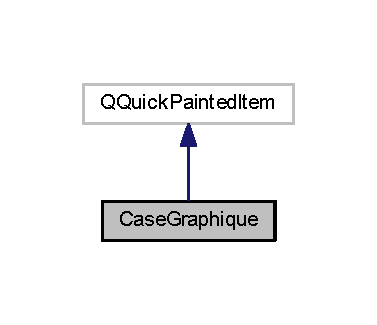
\includegraphics[width=181pt]{class_case_graphique__inherit__graph}
\end{center}
\end{figure}


Graphe de collaboration de Case\+Graphique\+:
\nopagebreak
\begin{figure}[H]
\begin{center}
\leavevmode
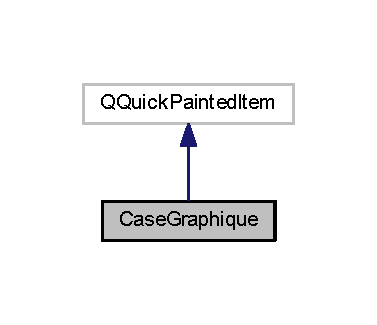
\includegraphics[width=181pt]{class_case_graphique__coll__graph}
\end{center}
\end{figure}
\subsection*{Connecteurs publics}
\begin{DoxyCompactItemize}
\item 
Q\+String {\bfseries couleur} ()\hypertarget{class_case_graphique_af731c72922e130f5a64c999badc03634}{}\label{class_case_graphique_af731c72922e130f5a64c999badc03634}

\item 
void {\bfseries set\+Couleur} (const Q\+String \&c)\hypertarget{class_case_graphique_a59b298e66484cfe89f62917f1f9b269b}{}\label{class_case_graphique_a59b298e66484cfe89f62917f1f9b269b}

\end{DoxyCompactItemize}
\subsection*{Signaux}
\begin{DoxyCompactItemize}
\item 
void {\bfseries couleur\+Changed} ()\hypertarget{class_case_graphique_a38480dc767a954d38aba3c2d8453a886}{}\label{class_case_graphique_a38480dc767a954d38aba3c2d8453a886}

\end{DoxyCompactItemize}
\subsection*{Fonctions membres publiques}
\begin{DoxyCompactItemize}
\item 
{\bfseries Case\+Graphique} (Q\+Quick\+Item $\ast$parent=0)\hypertarget{class_case_graphique_ac6a8ee4bfbd1e3c683066bae8157c41c}{}\label{class_case_graphique_ac6a8ee4bfbd1e3c683066bae8157c41c}

\item 
void {\bfseries paint} (Q\+Painter $\ast$painter)\hypertarget{class_case_graphique_a5ccb10775593928cfee6a4d5a5e9287c}{}\label{class_case_graphique_a5ccb10775593928cfee6a4d5a5e9287c}

\end{DoxyCompactItemize}
\subsection*{Attributs protégés}
\begin{DoxyCompactItemize}
\item 
Q\+Color {\bfseries m\+\_\+couleur}\hypertarget{class_case_graphique_ad2c0739e977728a58c6e8e8dc90440a0}{}\label{class_case_graphique_ad2c0739e977728a58c6e8e8dc90440a0}

\end{DoxyCompactItemize}
\subsection*{Propriétés}
\begin{DoxyCompactItemize}
\item 
Q\+String {\bfseries couleur}\hypertarget{class_case_graphique_abff90715a0c5492e141946eb99ee650a}{}\label{class_case_graphique_abff90715a0c5492e141946eb99ee650a}

\end{DoxyCompactItemize}


La documentation de cette classe a été générée à partir des fichiers suivants \+:\begin{DoxyCompactItemize}
\item 
src/\+Map/casegraphique.\+h\item 
src/\+Map/casegraphique.\+cpp\end{DoxyCompactItemize}

\hypertarget{class_case_map}{}\section{Référence de la classe Case\+Map}
\label{class_case_map}\index{Case\+Map@{Case\+Map}}


Graphe d\textquotesingle{}héritage de Case\+Map\+:
\nopagebreak
\begin{figure}[H]
\begin{center}
\leavevmode
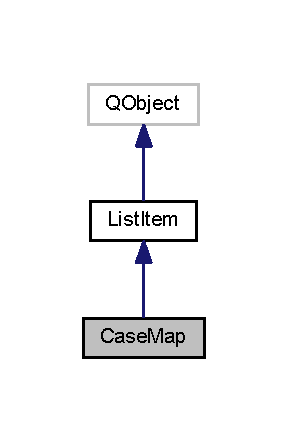
\includegraphics[width=138pt]{class_case_map__inherit__graph}
\end{center}
\end{figure}


Graphe de collaboration de Case\+Map\+:
\nopagebreak
\begin{figure}[H]
\begin{center}
\leavevmode
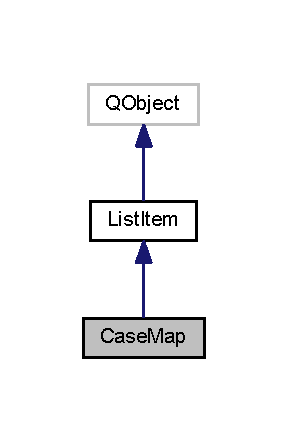
\includegraphics[width=138pt]{class_case_map__coll__graph}
\end{center}
\end{figure}
\subsection*{Types publics}
\begin{DoxyCompactItemize}
\item 
enum {\bfseries Roles} \{ {\bfseries Numero\+Role} = Qt\+:\+:User\+Role+1, 
{\bfseries Couleur\+Role}, 
{\bfseries Position\+X\+Role}, 
{\bfseries Position\+Y\+Role}
 \}\hypertarget{class_case_map_aeebf794e83d6f860b091b207b6ec6994}{}\label{class_case_map_aeebf794e83d6f860b091b207b6ec6994}

\end{DoxyCompactItemize}
\subsection*{Fonctions membres publiques}
\begin{DoxyCompactItemize}
\item 
{\bfseries Case\+Map} (Q\+Object $\ast$parent=0)\hypertarget{class_case_map_a2ce2f7eac32d04d1a3dd7bae6bfe49ef}{}\label{class_case_map_a2ce2f7eac32d04d1a3dd7bae6bfe49ef}

\item 
{\bfseries Case\+Map} (int name, const Q\+String \&couleur, Q\+Object $\ast$parent=0)\hypertarget{class_case_map_aa5992fb9f94916df679ba8924af1b402}{}\label{class_case_map_aa5992fb9f94916df679ba8924af1b402}

\item 
Q\+Variant {\bfseries data} (int role) const \hypertarget{class_case_map_aafb940559c3da7617a60d7e3c2c97b09}{}\label{class_case_map_aafb940559c3da7617a60d7e3c2c97b09}

\item 
Q\+Hash$<$ int, Q\+Byte\+Array $>$ {\bfseries role\+Names} () const \hypertarget{class_case_map_ae153e63fe7431386e61ea5993cf49099}{}\label{class_case_map_ae153e63fe7431386e61ea5993cf49099}

\item 
virtual bool {\bfseries set\+Data} (const Q\+Variant \&value, int role)\hypertarget{class_case_map_a1688bc1912122dfd309291a8e0596b95}{}\label{class_case_map_a1688bc1912122dfd309291a8e0596b95}

\item 
Q\+String {\bfseries id} () const \hypertarget{class_case_map_a787acbbce262bde9dca4fcd7c972c641}{}\label{class_case_map_a787acbbce262bde9dca4fcd7c972c641}

\item 
int {\bfseries numero} () const \hypertarget{class_case_map_a0e1a619a998369d054eca67d1b2035cb}{}\label{class_case_map_a0e1a619a998369d054eca67d1b2035cb}

\item 
Q\+String {\bfseries couleur} () const \hypertarget{class_case_map_a207917b31551bf6145598092f01abe0f}{}\label{class_case_map_a207917b31551bf6145598092f01abe0f}

\item 
int {\bfseries getX} () const \hypertarget{class_case_map_a65bd8c7a90488546b7a44da2a2a370b0}{}\label{class_case_map_a65bd8c7a90488546b7a44da2a2a370b0}

\item 
int {\bfseries getY} () const \hypertarget{class_case_map_a0a8910ab5161730d76e7d38cfd332ae1}{}\label{class_case_map_a0a8910ab5161730d76e7d38cfd332ae1}

\item 
bool {\bfseries setX} (int x)\hypertarget{class_case_map_a4b5ab60cc649cf779fca317e7701bab6}{}\label{class_case_map_a4b5ab60cc649cf779fca317e7701bab6}

\item 
bool {\bfseries setY} (int y)\hypertarget{class_case_map_a398a2dd2c220d42c8c0852b4c4b6bf4c}{}\label{class_case_map_a398a2dd2c220d42c8c0852b4c4b6bf4c}

\item 
bool {\bfseries set\+Couleur} (Q\+String couleur)\hypertarget{class_case_map_ab61c2e25a6ddcf59ddc57400caa31d48}{}\label{class_case_map_ab61c2e25a6ddcf59ddc57400caa31d48}

\end{DoxyCompactItemize}
\subsection*{Membres hérités additionnels}


La documentation de cette classe a été générée à partir des fichiers suivants \+:\begin{DoxyCompactItemize}
\item 
src/\+Map/case\+Map.\+h\item 
src/\+Map/case\+Map.\+cpp\end{DoxyCompactItemize}

\hypertarget{class_default}{}\section{Référence de la classe Default}
\label{class_default}\index{Default@{Default}}


Graphe d\textquotesingle{}héritage de Default\+:
\nopagebreak
\begin{figure}[H]
\begin{center}
\leavevmode
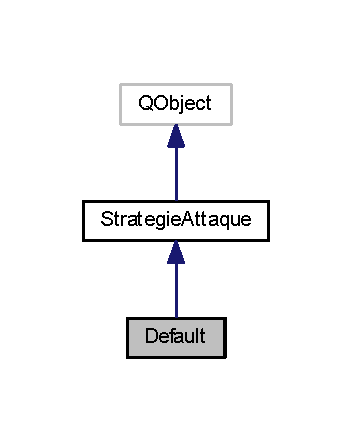
\includegraphics[width=169pt]{class_default__inherit__graph}
\end{center}
\end{figure}


Graphe de collaboration de Default\+:
\nopagebreak
\begin{figure}[H]
\begin{center}
\leavevmode
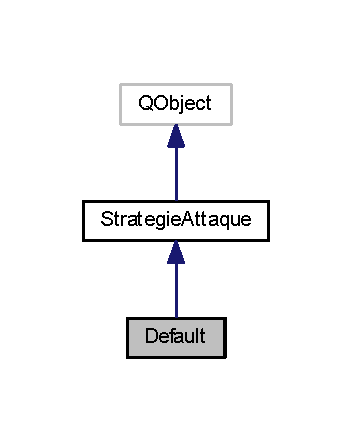
\includegraphics[width=169pt]{class_default__coll__graph}
\end{center}
\end{figure}
\subsection*{Fonctions membres publiques}
\begin{DoxyCompactItemize}
\item 
{\bfseries Default} (Q\+Object $\ast$parent=0)\hypertarget{class_default_ab11781e9e6e6a20708c1bf65a4f6da7e}{}\label{class_default_ab11781e9e6e6a20708c1bf65a4f6da7e}

\item 
virtual Q\+Point {\bfseries cibler} (const Q\+Vector$<$ Q\+Point $>$ $\ast$coup\+\_\+dispo, const Q\+Point \&map\+\_\+dimension)\hypertarget{class_default_a84280ded22bf749d9d11d59099cd02fd}{}\label{class_default_a84280ded22bf749d9d11d59099cd02fd}

\end{DoxyCompactItemize}


La documentation de cette classe a été générée à partir des fichiers suivants \+:\begin{DoxyCompactItemize}
\item 
src/strategie/default.\+h\item 
src/strategie/default.\+cpp\end{DoxyCompactItemize}

\hypertarget{class_difficile}{}\section{Référence de la classe Difficile}
\label{class_difficile}\index{Difficile@{Difficile}}


Graphe d\textquotesingle{}héritage de Difficile\+:
\nopagebreak
\begin{figure}[H]
\begin{center}
\leavevmode
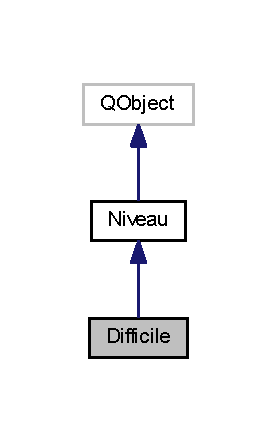
\includegraphics[width=133pt]{class_difficile__inherit__graph}
\end{center}
\end{figure}


Graphe de collaboration de Difficile\+:
\nopagebreak
\begin{figure}[H]
\begin{center}
\leavevmode
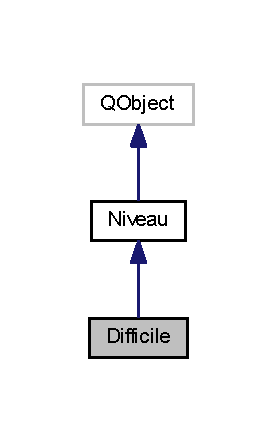
\includegraphics[width=133pt]{class_difficile__coll__graph}
\end{center}
\end{figure}
\subsection*{Fonctions membres publiques}
\begin{DoxyCompactItemize}
\item 
{\bfseries Difficile} (Q\+Object $\ast$parent)\hypertarget{class_difficile_a0231ef40e1ded703a0cdfdf19eb91514}{}\label{class_difficile_a0231ef40e1ded703a0cdfdf19eb91514}

\item 
virtual int {\bfseries resistance\+Navire\+Ordi} ()\hypertarget{class_difficile_af3a6bab0cdcd63d9be464c0c4e07cb66}{}\label{class_difficile_af3a6bab0cdcd63d9be464c0c4e07cb66}

\item 
virtual int {\bfseries resistance\+Navire\+Joueur} ()\hypertarget{class_difficile_ab9b40f803d46477a49db5c7ad4974436}{}\label{class_difficile_ab9b40f803d46477a49db5c7ad4974436}

\end{DoxyCompactItemize}
\subsection*{Membres hérités additionnels}


La documentation de cette classe a été générée à partir des fichiers suivants \+:\begin{DoxyCompactItemize}
\item 
src/niveau/difficile.\+h\item 
src/niveau/difficile.\+cpp\end{DoxyCompactItemize}

\hypertarget{class_en_croix}{}\section{Référence de la classe En\+Croix}
\label{class_en_croix}\index{En\+Croix@{En\+Croix}}


Graphe d\textquotesingle{}héritage de En\+Croix\+:
\nopagebreak
\begin{figure}[H]
\begin{center}
\leavevmode
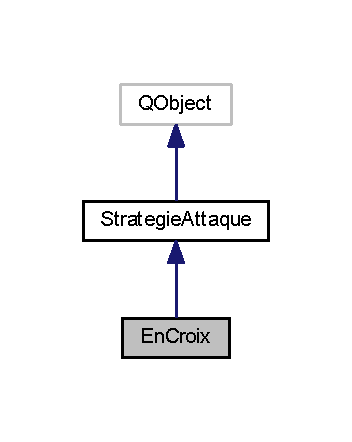
\includegraphics[width=169pt]{class_en_croix__inherit__graph}
\end{center}
\end{figure}


Graphe de collaboration de En\+Croix\+:
\nopagebreak
\begin{figure}[H]
\begin{center}
\leavevmode
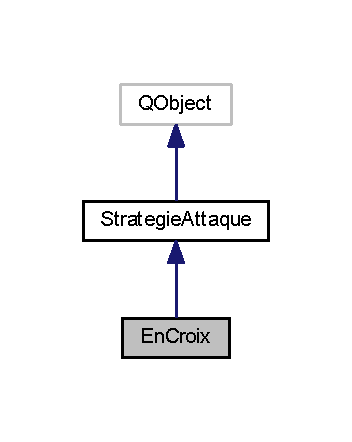
\includegraphics[width=169pt]{class_en_croix__coll__graph}
\end{center}
\end{figure}
\subsection*{Fonctions membres publiques}
\begin{DoxyCompactItemize}
\item 
{\bfseries En\+Croix} (Q\+Object $\ast$parent=0)\hypertarget{class_en_croix_a2d45294635fb84fd174b4f46a8e3fba2}{}\label{class_en_croix_a2d45294635fb84fd174b4f46a8e3fba2}

\item 
virtual Q\+Point {\bfseries cibler} (const Q\+Vector$<$ Q\+Point $>$ $\ast$coup\+\_\+dispo, const Q\+Point \&map\+\_\+dimension)\hypertarget{class_en_croix_a7a93757f1d6b75c6e00c694a39cf3a85}{}\label{class_en_croix_a7a93757f1d6b75c6e00c694a39cf3a85}

\end{DoxyCompactItemize}
\subsection*{Attributs protégés}
\begin{DoxyCompactItemize}
\item 
Q\+Point {\bfseries m\+\_\+last} = Q\+Point( I\+N\+T\+\_\+\+M\+AX-\/2, I\+N\+T\+\_\+\+M\+AX-\/2)\hypertarget{class_en_croix_a526cf92dd33b7cf2f27c48ec1b9e6ffe}{}\label{class_en_croix_a526cf92dd33b7cf2f27c48ec1b9e6ffe}

\end{DoxyCompactItemize}


La documentation de cette classe a été générée à partir des fichiers suivants \+:\begin{DoxyCompactItemize}
\item 
src/strategie/encroix.\+h\item 
src/strategie/encroix.\+cpp\end{DoxyCompactItemize}

\hypertarget{class_enligne}{}\section{Référence de la classe Enligne}
\label{class_enligne}\index{Enligne@{Enligne}}


Graphe d\textquotesingle{}héritage de Enligne\+:
\nopagebreak
\begin{figure}[H]
\begin{center}
\leavevmode
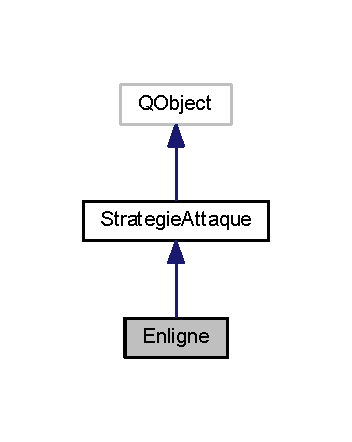
\includegraphics[width=169pt]{class_enligne__inherit__graph}
\end{center}
\end{figure}


Graphe de collaboration de Enligne\+:
\nopagebreak
\begin{figure}[H]
\begin{center}
\leavevmode
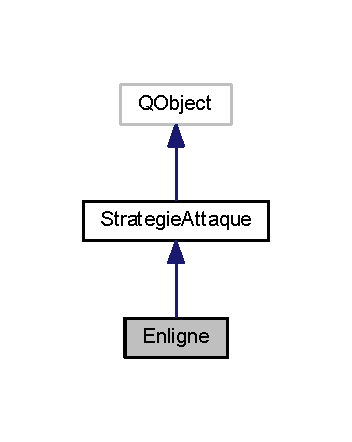
\includegraphics[width=169pt]{class_enligne__coll__graph}
\end{center}
\end{figure}
\subsection*{Fonctions membres publiques}
\begin{DoxyCompactItemize}
\item 
{\bfseries Enligne} (Q\+Object $\ast$parent=0)\hypertarget{class_enligne_afaa0cfcd78b2b04e2ba6d5fe54ab371f}{}\label{class_enligne_afaa0cfcd78b2b04e2ba6d5fe54ab371f}

\item 
virtual Q\+Point {\bfseries cibler} (const Q\+Vector$<$ Q\+Point $>$ $\ast$coup\+\_\+dispo, const Q\+Point \&map\+\_\+dimension)\hypertarget{class_enligne_ab4935689fd3ca6a0d4a351929b120493}{}\label{class_enligne_ab4935689fd3ca6a0d4a351929b120493}

\end{DoxyCompactItemize}
\subsection*{Attributs protégés}
\begin{DoxyCompactItemize}
\item 
Q\+Point {\bfseries m\+\_\+last} = Q\+Point( I\+N\+T\+\_\+\+M\+AX-\/2, I\+N\+T\+\_\+\+M\+AX-\/2)\hypertarget{class_enligne_a7b15585630a7b29388900e30a2ed33fe}{}\label{class_enligne_a7b15585630a7b29388900e30a2ed33fe}

\end{DoxyCompactItemize}


La documentation de cette classe a été générée à partir des fichiers suivants \+:\begin{DoxyCompactItemize}
\item 
src/strategie/enligne.\+h\item 
src/strategie/enligne.\+cpp\end{DoxyCompactItemize}

\hypertarget{class_facile}{}\section{Référence de la classe Facile}
\label{class_facile}\index{Facile@{Facile}}


Graphe d\textquotesingle{}héritage de Facile\+:
\nopagebreak
\begin{figure}[H]
\begin{center}
\leavevmode
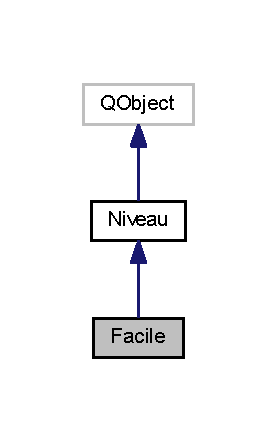
\includegraphics[width=133pt]{class_facile__inherit__graph}
\end{center}
\end{figure}


Graphe de collaboration de Facile\+:
\nopagebreak
\begin{figure}[H]
\begin{center}
\leavevmode
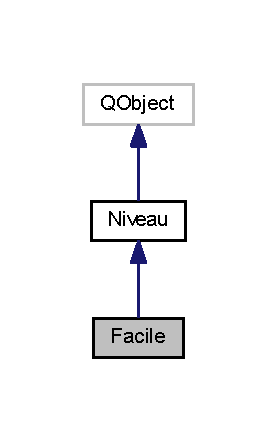
\includegraphics[width=133pt]{class_facile__coll__graph}
\end{center}
\end{figure}
\subsection*{Fonctions membres publiques}
\begin{DoxyCompactItemize}
\item 
{\bfseries Facile} (Q\+Object $\ast$parent=0)\hypertarget{class_facile_ab7147028ffb0ff80075d886fc173e471}{}\label{class_facile_ab7147028ffb0ff80075d886fc173e471}

\item 
virtual int {\bfseries resistance\+Navire\+Ordi} ()\hypertarget{class_facile_adb34e5aa4d1a2ae642496324c6df3495}{}\label{class_facile_adb34e5aa4d1a2ae642496324c6df3495}

\item 
virtual int {\bfseries resistance\+Navire\+Joueur} ()\hypertarget{class_facile_aa1f252c0a75eec896b11783f76b2ffbf}{}\label{class_facile_aa1f252c0a75eec896b11783f76b2ffbf}

\end{DoxyCompactItemize}
\subsection*{Membres hérités additionnels}


La documentation de cette classe a été générée à partir des fichiers suivants \+:\begin{DoxyCompactItemize}
\item 
src/niveau/facile.\+h\item 
src/niveau/facile.\+cpp\end{DoxyCompactItemize}

\hypertarget{class_factory_mosaique}{}\section{Référence de la classe Factory\+Mosaique}
\label{class_factory_mosaique}\index{Factory\+Mosaique@{Factory\+Mosaique}}


Graphe d\textquotesingle{}héritage de Factory\+Mosaique\+:
\nopagebreak
\begin{figure}[H]
\begin{center}
\leavevmode
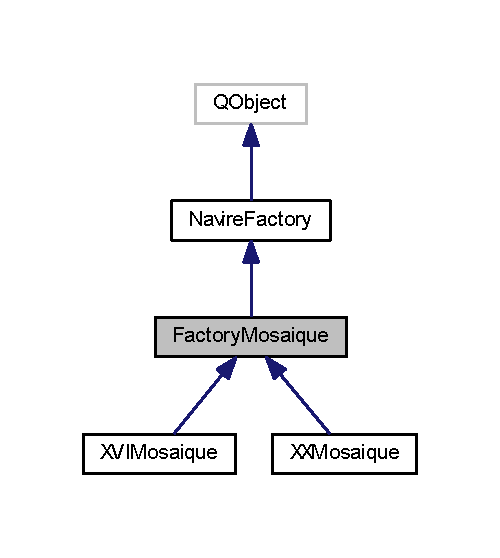
\includegraphics[width=240pt]{class_factory_mosaique__inherit__graph}
\end{center}
\end{figure}


Graphe de collaboration de Factory\+Mosaique\+:
\nopagebreak
\begin{figure}[H]
\begin{center}
\leavevmode
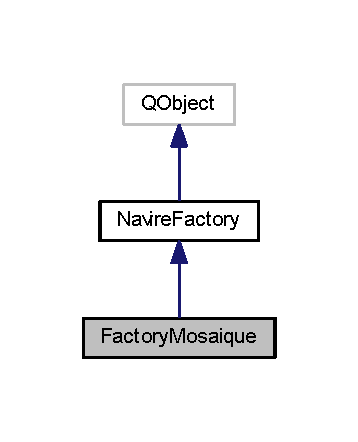
\includegraphics[width=172pt]{class_factory_mosaique__coll__graph}
\end{center}
\end{figure}
\subsection*{Fonctions membres publiques}
\begin{DoxyCompactItemize}
\item 
{\bfseries Factory\+Mosaique} (Q\+Object $\ast$parent=0)\hypertarget{class_factory_mosaique_aa0cdf96f0abd1623e63c81c268b15bb9}{}\label{class_factory_mosaique_aa0cdf96f0abd1623e63c81c268b15bb9}

\item 
virtual Q\+List$<$ \hyperlink{class_navire}{Navire} $\ast$ $>$ {\bfseries creer\+Navire} (int nombre, int resistance\+Navire)\hypertarget{class_factory_mosaique_ac0ccf73da963831249e504287e3c8d94}{}\label{class_factory_mosaique_ac0ccf73da963831249e504287e3c8d94}

\item 
virtual \hyperlink{class_navire2_d}{Navire2D} $\ast$ {\bfseries nouveau\+Navire2D} (int resistance\+Navire)=0\hypertarget{class_factory_mosaique_a68a26f2ad764f31e1bf03576a841808b}{}\label{class_factory_mosaique_a68a26f2ad764f31e1bf03576a841808b}

\item 
virtual \hyperlink{class_navire3_d}{Navire3D} $\ast$ {\bfseries nouveau\+Navire3D} (int resistance\+Navire)=0\hypertarget{class_factory_mosaique_a6028cfbc8fdc3825db31f39973ec9ebd}{}\label{class_factory_mosaique_a6028cfbc8fdc3825db31f39973ec9ebd}

\item 
virtual \hyperlink{class_navire4_d}{Navire4D} $\ast$ {\bfseries nouveau\+Navire4D} (int resistance\+Navire)=0\hypertarget{class_factory_mosaique_ac2adb008a36298015b47f32b2e58c25a}{}\label{class_factory_mosaique_ac2adb008a36298015b47f32b2e58c25a}

\end{DoxyCompactItemize}
\subsection*{Membres hérités additionnels}


La documentation de cette classe a été générée à partir des fichiers suivants \+:\begin{DoxyCompactItemize}
\item 
src/\+Global/navire\+Factory/factorymosaique.\+h\item 
src/\+Global/navire\+Factory/factorymosaique.\+cpp\end{DoxyCompactItemize}

\hypertarget{class_joueur}{}\section{Référence de la classe Joueur}
\label{class_joueur}\index{Joueur@{Joueur}}


Graphe d\textquotesingle{}héritage de Joueur\+:
\nopagebreak
\begin{figure}[H]
\begin{center}
\leavevmode
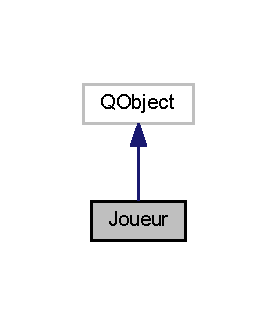
\includegraphics[width=133pt]{class_joueur__inherit__graph}
\end{center}
\end{figure}


Graphe de collaboration de Joueur\+:
\nopagebreak
\begin{figure}[H]
\begin{center}
\leavevmode
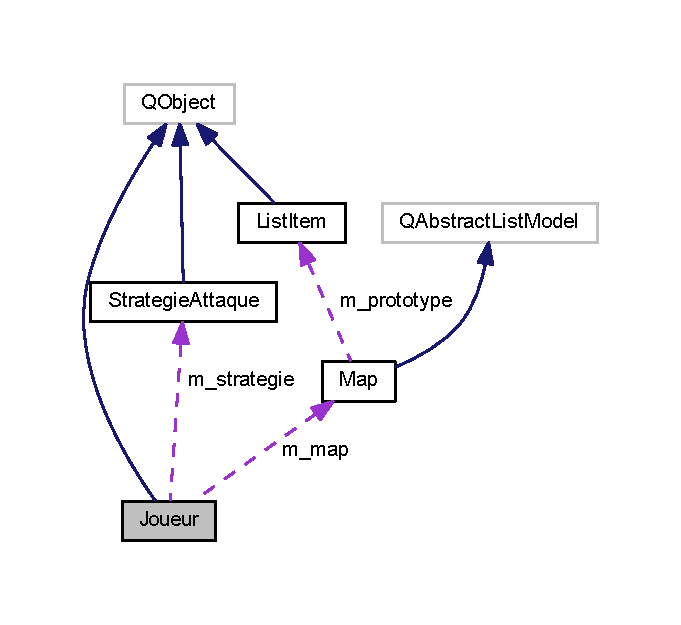
\includegraphics[width=327pt]{class_joueur__coll__graph}
\end{center}
\end{figure}
\subsection*{Classes}
\begin{DoxyCompactItemize}
\item 
struct \hyperlink{struct_joueur_1_1_position}{Position}
\end{DoxyCompactItemize}
\subsection*{Connecteurs publics}
\begin{DoxyCompactItemize}
\item 
Q\+\_\+\+I\+N\+V\+O\+K\+A\+B\+LE Q\+Variant {\bfseries get\+Next\+Navire\+A\+Placer} ()\hypertarget{class_joueur_ab5bdd0ac7f43d430a91ed9521d92cacd}{}\label{class_joueur_ab5bdd0ac7f43d430a91ed9521d92cacd}

\item 
const Q\+Variant {\bfseries get\+List\+Navire} () const \hypertarget{class_joueur_aa8dc64eecabea9282cc6bc7634434cbd}{}\label{class_joueur_aa8dc64eecabea9282cc6bc7634434cbd}

\item 
Q\+\_\+\+I\+N\+V\+O\+K\+A\+B\+LE bool {\bfseries est\+Humain} ()\hypertarget{class_joueur_ac9330f6d335cdb5ad1a50a292945135d}{}\label{class_joueur_ac9330f6d335cdb5ad1a50a292945135d}

\item 
int {\bfseries position\+X\+Navire} (\hyperlink{class_navire}{Navire} $\ast$navire) const \hypertarget{class_joueur_a700a86d9e204507bc67f4aa2d8ab26a8}{}\label{class_joueur_a700a86d9e204507bc67f4aa2d8ab26a8}

\item 
int {\bfseries position\+Y\+Navire} (\hyperlink{class_navire}{Navire} $\ast$navire) const \hypertarget{class_joueur_a902dbe595e80886dd8d26a06be2c4fa6}{}\label{class_joueur_a902dbe595e80886dd8d26a06be2c4fa6}

\item 
void {\bfseries placer\+Navire} (\hyperlink{class_navire}{Navire} $\ast$navire, Q\+List$<$ int $>$ cases, bool horizontale)\hypertarget{class_joueur_a64d0164fe784e5f348612cd536ab86f4}{}\label{class_joueur_a64d0164fe784e5f348612cd536ab86f4}

\item 
int {\bfseries nb\+Navire} ()\hypertarget{class_joueur_a26d44b10a21dad6e35ab26e6556071bf}{}\label{class_joueur_a26d44b10a21dad6e35ab26e6556071bf}

\end{DoxyCompactItemize}
\subsection*{Signaux}
\begin{DoxyCompactItemize}
\item 
void {\bfseries nb\+Navire\+Changed} ()\hypertarget{class_joueur_a18aaca01f9653ea6626e40367d75dde4}{}\label{class_joueur_a18aaca01f9653ea6626e40367d75dde4}

\item 
void {\bfseries navire\+Partie\+Detruite} (int position, Q\+Point pos)\hypertarget{class_joueur_aaf57fa0209c5e5e9ec62cf4a544cd77d}{}\label{class_joueur_aaf57fa0209c5e5e9ec62cf4a544cd77d}

\item 
void {\bfseries attaque\+Subit\+Rate} (int position, Q\+Point pos)\hypertarget{class_joueur_af7f12644d0e0aefaa136d0e2839b386f}{}\label{class_joueur_af7f12644d0e0aefaa136d0e2839b386f}

\end{DoxyCompactItemize}
\subsection*{Fonctions membres publiques}
\begin{DoxyCompactItemize}
\item 
{\bfseries Joueur} (Q\+String identifiant, \hyperlink{class_navire_factory}{Navire\+Factory} $\ast$navire\+Factory, int nb\+\_\+navire, int resistance\+Navire, bool humain=true, Q\+Object $\ast$parent=0)\hypertarget{class_joueur_a0f254ef9e5c9a22dc174fa4672078242}{}\label{class_joueur_a0f254ef9e5c9a22dc174fa4672078242}

\item 
bool \hyperlink{class_joueur_afe82d80d5b5f48f40de36cbd420dcab1}{add\+Case} (\hyperlink{class_navire}{Navire} $\ast$navire, Q\+List$<$ int $>$ \&cases)
\begin{DoxyCompactList}\small\item\em add\+Case ajoute le navire avec ses cases associées dans la collection des navires du joueur \end{DoxyCompactList}\item 
void {\bfseries placement\+Automatique} ()\hypertarget{class_joueur_a582ea6ef1f7cd5a6d2259958e34f181a}{}\label{class_joueur_a582ea6ef1f7cd5a6d2259958e34f181a}

\item 
void {\bfseries creer\+Map} (Q\+Point dimension)\hypertarget{class_joueur_a615622a48fb0da97f7015ec35826c418}{}\label{class_joueur_a615622a48fb0da97f7015ec35826c418}

\item 
bool \hyperlink{class_joueur_a6dff19070bdd6e9f1fdbac056a563b08}{recevoir\+Attaque} (int position, int mon\+\_\+index)
\begin{DoxyCompactList}\small\item\em \hyperlink{class_joueur_a6dff19070bdd6e9f1fdbac056a563b08}{Joueur\+::recevoir\+Attaque}. \end{DoxyCompactList}\item 
int {\bfseries attaque\+Automatique} (const Q\+Vector$<$ Q\+Point $>$ $\ast$coup, Q\+Point \&position)\hypertarget{class_joueur_a679e730ac2c283452a818e83b02c1990}{}\label{class_joueur_a679e730ac2c283452a818e83b02c1990}

\item 
void {\bfseries set\+Strategie} (Q\+String strategie)\hypertarget{class_joueur_ac10802f705a39547e7433cffbcd901e1}{}\label{class_joueur_ac10802f705a39547e7433cffbcd901e1}

\item 
{\bfseries operator Q\+String} () const \hypertarget{class_joueur_ad6f3af78b8c26e447f218c31f5278845}{}\label{class_joueur_ad6f3af78b8c26e447f218c31f5278845}

\item 
Q\+String {\bfseries identifiant} ()\hypertarget{class_joueur_a72d82a284c89ae702dd1bc352284f65f}{}\label{class_joueur_a72d82a284c89ae702dd1bc352284f65f}

\end{DoxyCompactItemize}
\subsection*{Fonctions membres protégées}
\begin{DoxyCompactItemize}
\item 
const Q\+Variant {\bfseries get\+Map} () const \hypertarget{class_joueur_a835c64ce76ce21f8baa7bbf9bdb32612}{}\label{class_joueur_a835c64ce76ce21f8baa7bbf9bdb32612}

\end{DoxyCompactItemize}
\subsection*{Attributs protégés}
\begin{DoxyCompactItemize}
\item 
Q\+Hash$<$ Q\+Object $\ast$, \hyperlink{struct_joueur_1_1_position}{Position} $>$ {\bfseries m\+\_\+navires}\hypertarget{class_joueur_aba03135ccdc3901ba8199c2f07b42126}{}\label{class_joueur_aba03135ccdc3901ba8199c2f07b42126}

\item 
\hyperlink{class_strategie_attaque}{Strategie\+Attaque} $\ast$ {\bfseries m\+\_\+strategie} = nullptr\hypertarget{class_joueur_ab5e526d57bc6cd5809f7443b72d4b45c}{}\label{class_joueur_ab5e526d57bc6cd5809f7443b72d4b45c}

\item 
Q\+List$<$ \hyperlink{class_navire}{Navire} $\ast$ $>$ {\bfseries m\+\_\+liste}\hypertarget{class_joueur_a5959e2f19a5a8eba223dde5cebcd3024}{}\label{class_joueur_a5959e2f19a5a8eba223dde5cebcd3024}

\item 
bool {\bfseries m\+\_\+humain}\hypertarget{class_joueur_a557ffbf046f630836151477dd729f829}{}\label{class_joueur_a557ffbf046f630836151477dd729f829}

\item 
\hyperlink{class_map}{Map} $\ast$ {\bfseries m\+\_\+map} = nullptr\hypertarget{class_joueur_af8523f4d4f659e4e1b66a2e4e7a54930}{}\label{class_joueur_af8523f4d4f659e4e1b66a2e4e7a54930}

\item 
Q\+String {\bfseries m\+\_\+identifiant}\hypertarget{class_joueur_a84c7d5ca2764bb11b7034069d07ff951}{}\label{class_joueur_a84c7d5ca2764bb11b7034069d07ff951}

\end{DoxyCompactItemize}
\subsection*{Propriétés}
\begin{DoxyCompactItemize}
\item 
Q\+Variant {\bfseries map}\hypertarget{class_joueur_ab5cad2e942f337bae4349169ff26fe75}{}\label{class_joueur_ab5cad2e942f337bae4349169ff26fe75}

\item 
int {\bfseries nb\+Navire}\hypertarget{class_joueur_a6d2112156c9b08e9c8be56d3db8433ee}{}\label{class_joueur_a6d2112156c9b08e9c8be56d3db8433ee}

\item 
Q\+String {\bfseries identifiant}\hypertarget{class_joueur_a723d1011cd81c14c8b43843a52d9bdbd}{}\label{class_joueur_a723d1011cd81c14c8b43843a52d9bdbd}

\end{DoxyCompactItemize}


\subsection{Documentation des fonctions membres}
\index{Joueur@{Joueur}!add\+Case@{add\+Case}}
\index{add\+Case@{add\+Case}!Joueur@{Joueur}}
\subsubsection[{\texorpdfstring{add\+Case(\+Navire $\ast$navire, Q\+List$<$ int $>$ \&cases)}{addCase(Navire *navire, QList< int > &cases)}}]{\setlength{\rightskip}{0pt plus 5cm}bool Joueur\+::add\+Case (
\begin{DoxyParamCaption}
\item[{{\bf Navire} $\ast$}]{navire, }
\item[{Q\+List$<$ int $>$ \&}]{cases}
\end{DoxyParamCaption}
)}\hypertarget{class_joueur_afe82d80d5b5f48f40de36cbd420dcab1}{}\label{class_joueur_afe82d80d5b5f48f40de36cbd420dcab1}


add\+Case ajoute le navire avec ses cases associées dans la collection des navires du joueur 

\begin{DoxyReturn}{Renvoie}
true si le navire a bien été ajouté 
\end{DoxyReturn}
\index{Joueur@{Joueur}!recevoir\+Attaque@{recevoir\+Attaque}}
\index{recevoir\+Attaque@{recevoir\+Attaque}!Joueur@{Joueur}}
\subsubsection[{\texorpdfstring{recevoir\+Attaque(int position, int mon\+\_\+index)}{recevoirAttaque(int position, int mon_index)}}]{\setlength{\rightskip}{0pt plus 5cm}bool Joueur\+::recevoir\+Attaque (
\begin{DoxyParamCaption}
\item[{int}]{position, }
\item[{int}]{mon\+\_\+index}
\end{DoxyParamCaption}
)}\hypertarget{class_joueur_a6dff19070bdd6e9f1fdbac056a563b08}{}\label{class_joueur_a6dff19070bdd6e9f1fdbac056a563b08}


\hyperlink{class_joueur_a6dff19070bdd6e9f1fdbac056a563b08}{Joueur\+::recevoir\+Attaque}. 


\begin{DoxyParams}{Paramètres}
{\em position} & \\
\hline
\end{DoxyParams}
\begin{DoxyReturn}{Renvoie}
true si le joueur cible est mort 
\end{DoxyReturn}


La documentation de cette classe a été générée à partir des fichiers suivants \+:\begin{DoxyCompactItemize}
\item 
src/\+Global/joueur.\+h\item 
src/\+Global/joueur.\+cpp\end{DoxyCompactItemize}

\hypertarget{class_launcher}{}\section{Référence de la classe Launcher}
\label{class_launcher}\index{Launcher@{Launcher}}


Graphe d\textquotesingle{}héritage de Launcher\+:
\nopagebreak
\begin{figure}[H]
\begin{center}
\leavevmode
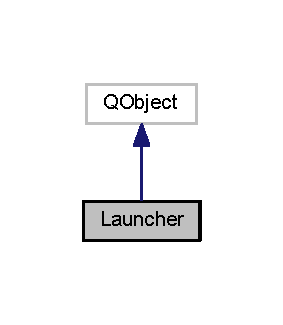
\includegraphics[width=136pt]{class_launcher__inherit__graph}
\end{center}
\end{figure}


Graphe de collaboration de Launcher\+:
\nopagebreak
\begin{figure}[H]
\begin{center}
\leavevmode
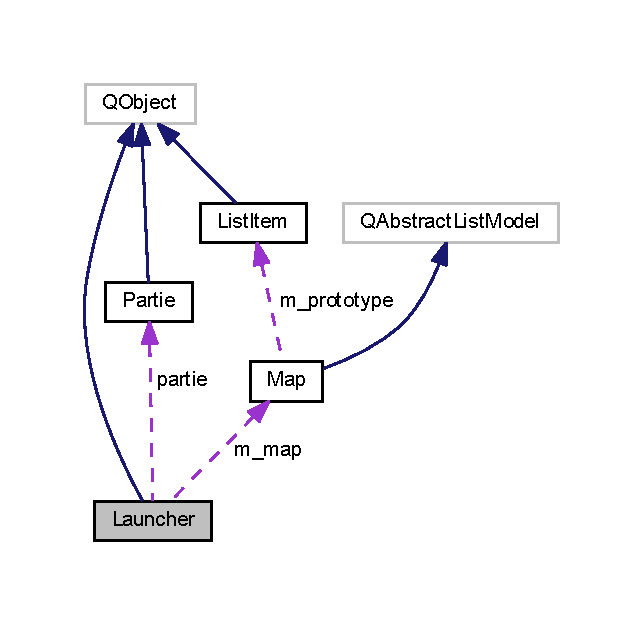
\includegraphics[width=308pt]{class_launcher__coll__graph}
\end{center}
\end{figure}
\subsection*{Connecteurs publics}
\begin{DoxyCompactItemize}
\item 
Q\+Variant {\bfseries niveau} ()\hypertarget{class_launcher_a066cf8162322b8c548a5374ffd91a065}{}\label{class_launcher_a066cf8162322b8c548a5374ffd91a065}

\item 
int {\bfseries index\+\_\+niveau} ()\hypertarget{class_launcher_a615138eaf9a49eff6cecda2be7145f96}{}\label{class_launcher_a615138eaf9a49eff6cecda2be7145f96}

\item 
void {\bfseries set\+Index\+\_\+niveau} (int i)\hypertarget{class_launcher_afa0d73c92ab966138c515b40d1b4ed3d}{}\label{class_launcher_afa0d73c92ab966138c515b40d1b4ed3d}

\item 
int {\bfseries mode} ()\hypertarget{class_launcher_affbdb351a7da8ae1e9030084ed3f4fd6}{}\label{class_launcher_affbdb351a7da8ae1e9030084ed3f4fd6}

\item 
void {\bfseries set\+Mode} (Q\+String mode)\hypertarget{class_launcher_a06b9eca9d74aae8a03b46b5bde878fe4}{}\label{class_launcher_a06b9eca9d74aae8a03b46b5bde878fe4}

\item 
int {\bfseries epoque} ()\hypertarget{class_launcher_a78cf7830a87925184255033388bef731}{}\label{class_launcher_a78cf7830a87925184255033388bef731}

\item 
void {\bfseries set\+Epoque} (Q\+String epoque)\hypertarget{class_launcher_ad6df98ebd2924b167e64f9a9fedd98e2}{}\label{class_launcher_ad6df98ebd2924b167e64f9a9fedd98e2}

\item 
bool {\bfseries placement} ()\hypertarget{class_launcher_ac0837d73a6998d55be80daab8fa46c6d}{}\label{class_launcher_ac0837d73a6998d55be80daab8fa46c6d}

\item 
void {\bfseries set\+Placement} (bool b)\hypertarget{class_launcher_a4879d5ff3d4abc22cb14ce1caf46a3e5}{}\label{class_launcher_a4879d5ff3d4abc22cb14ce1caf46a3e5}

\item 
int {\bfseries nombre\+\_\+navire} ()\hypertarget{class_launcher_abc6ea53613b21dabd9d17c0264e55c74}{}\label{class_launcher_abc6ea53613b21dabd9d17c0264e55c74}

\item 
Q\+\_\+\+I\+N\+V\+O\+K\+A\+B\+LE const Q\+String\+List {\bfseries get\+Liste\+Mode} () const \hypertarget{class_launcher_aa5a95be43fa5e9c893ac63497dc33b62}{}\label{class_launcher_aa5a95be43fa5e9c893ac63497dc33b62}

\item 
Q\+\_\+\+I\+N\+V\+O\+K\+A\+B\+LE const Q\+String\+List {\bfseries get\+Liste\+Epoque} () const \hypertarget{class_launcher_a1d72251df85672b9990bb4eb29864cd9}{}\label{class_launcher_a1d72251df85672b9990bb4eb29864cd9}

\item 
Q\+\_\+\+I\+N\+V\+O\+K\+A\+B\+LE void {\bfseries start} ()\hypertarget{class_launcher_a31ee0ccbd35abeaa5b78b4d330278ca3}{}\label{class_launcher_a31ee0ccbd35abeaa5b78b4d330278ca3}

\end{DoxyCompactItemize}
\subsection*{Signaux}
\begin{DoxyCompactItemize}
\item 
void {\bfseries niveau\+Changed} ()\hypertarget{class_launcher_ab1f9224509580eba78c05741aefca0bd}{}\label{class_launcher_ab1f9224509580eba78c05741aefca0bd}

\item 
void {\bfseries placement\+Changed} ()\hypertarget{class_launcher_af3a5eb7de657dfa21c0c26b8dbd8ca07}{}\label{class_launcher_af3a5eb7de657dfa21c0c26b8dbd8ca07}

\item 
void {\bfseries partie\+Changed} ()\hypertarget{class_launcher_aa0ee62bf97439fb86c6c6c70de06592e}{}\label{class_launcher_aa0ee62bf97439fb86c6c6c70de06592e}

\item 
void {\bfseries strategie\+Changed} ()\hypertarget{class_launcher_a52fa53afdcf2f4acace21f011fba6532}{}\label{class_launcher_a52fa53afdcf2f4acace21f011fba6532}

\item 
void {\bfseries nombre\+\_\+navire\+Changed} ()\hypertarget{class_launcher_a4c707e424f1f193ce92d2c9768f774db}{}\label{class_launcher_a4c707e424f1f193ce92d2c9768f774db}

\end{DoxyCompactItemize}
\subsection*{Fonctions membres publiques}
\begin{DoxyCompactItemize}
\item 
{\bfseries Launcher} (Q\+Qml\+Application\+Engine $\ast$engine, Q\+Object $\ast$parent=0)\hypertarget{class_launcher_acbbd874223d4de183d20635d8cd65f44}{}\label{class_launcher_acbbd874223d4de183d20635d8cd65f44}

\end{DoxyCompactItemize}
\subsection*{Fonctions membres protégées}
\begin{DoxyCompactItemize}
\item 
void {\bfseries set\+Strategie} (Q\+String s)\hypertarget{class_launcher_a275bb65345df87d43fb618bf9a586ed7}{}\label{class_launcher_a275bb65345df87d43fb618bf9a586ed7}

\item 
Q\+String {\bfseries strategie} ()\hypertarget{class_launcher_a997d7229e1aec8b3ef3901cdb1bb9c72}{}\label{class_launcher_a997d7229e1aec8b3ef3901cdb1bb9c72}

\item 
void {\bfseries set\+Nombre\+\_\+navire} (int i)\hypertarget{class_launcher_a39ca36b788d9b2ce1ee530f2be10d1ff}{}\label{class_launcher_a39ca36b788d9b2ce1ee530f2be10d1ff}

\end{DoxyCompactItemize}
\subsection*{Attributs protégés}
\begin{DoxyCompactItemize}
\item 
Q\+List$<$ Q\+Object $\ast$ $>$ {\bfseries m\+\_\+liste\+Niveau}\hypertarget{class_launcher_aad53e1b71b8a75e1750dcfaa4865bd1c}{}\label{class_launcher_aad53e1b71b8a75e1750dcfaa4865bd1c}

\item 
int {\bfseries m\+\_\+index\+\_\+niveau} = 0\hypertarget{class_launcher_a907c78bc7fee7c8a909b74caed883f6e}{}\label{class_launcher_a907c78bc7fee7c8a909b74caed883f6e}

\item 
\hyperlink{class_partie}{Partie} $\ast$ {\bfseries partie} = nullptr\hypertarget{class_launcher_a9a3398a253707bf673e984c87f8ab6ad}{}\label{class_launcher_a9a3398a253707bf673e984c87f8ab6ad}

\item 
Navire\+Factory\+::\+Type {\bfseries m\+\_\+mode}\hypertarget{class_launcher_a54bbd14816ad4c6b140e9aceb5d2e795}{}\label{class_launcher_a54bbd14816ad4c6b140e9aceb5d2e795}

\item 
Navire\+Factory\+::\+Epoque {\bfseries m\+\_\+epoque} = Navire\+Factory\+::\+Epoque\+::\+XX\hypertarget{class_launcher_a5eb8d3986315d6a5cc9abd2bbfaa41a1}{}\label{class_launcher_a5eb8d3986315d6a5cc9abd2bbfaa41a1}

\item 
int {\bfseries m\+\_\+nb\+Navire} = 3\hypertarget{class_launcher_aeda234c735529c97812a69f3470dbcc9}{}\label{class_launcher_aeda234c735529c97812a69f3470dbcc9}

\item 
Q\+String {\bfseries m\+\_\+strategie} = \char`\"{}default\char`\"{}\hypertarget{class_launcher_a9e01a5476729d03a4f806f06cbf551bd}{}\label{class_launcher_a9e01a5476729d03a4f806f06cbf551bd}

\item 
bool {\bfseries m\+\_\+placement} = false\hypertarget{class_launcher_a54392937a9852e1efc37287e8943eafd}{}\label{class_launcher_a54392937a9852e1efc37287e8943eafd}

\item 
Q\+Qml\+Application\+Engine $\ast$ {\bfseries m\+\_\+engine}\hypertarget{class_launcher_abfdd9c4e05cb09342c8e2dfee924b339}{}\label{class_launcher_abfdd9c4e05cb09342c8e2dfee924b339}

\item 
Q\+Point {\bfseries m\+\_\+dimensions} = Q\+Point(10,10)\hypertarget{class_launcher_aeb5da8a5148fcb0dad2583536bedb235}{}\label{class_launcher_aeb5da8a5148fcb0dad2583536bedb235}

\item 
\hyperlink{class_map}{Map} $\ast$ {\bfseries m\+\_\+map} = nullptr\hypertarget{class_launcher_a27f701fa3cc5c82cdf77746997ed4f95}{}\label{class_launcher_a27f701fa3cc5c82cdf77746997ed4f95}

\end{DoxyCompactItemize}
\subsection*{Propriétés}
\begin{DoxyCompactItemize}
\item 
Q\+Variant {\bfseries niveau}\hypertarget{class_launcher_a5a179c1054360e4a9ed4ed7ab68bc669}{}\label{class_launcher_a5a179c1054360e4a9ed4ed7ab68bc669}

\item 
int {\bfseries index\+\_\+niveau}\hypertarget{class_launcher_a3d11ce16022d3be36e2d08d16bce7a20}{}\label{class_launcher_a3d11ce16022d3be36e2d08d16bce7a20}

\item 
bool {\bfseries placement}\hypertarget{class_launcher_a66757e33dc479289c6717e0026013827}{}\label{class_launcher_a66757e33dc479289c6717e0026013827}

\item 
Q\+String {\bfseries strategie}\hypertarget{class_launcher_a6c6261cfe4560a48e66f9144613098b6}{}\label{class_launcher_a6c6261cfe4560a48e66f9144613098b6}

\item 
int {\bfseries nombre\+\_\+navire}\hypertarget{class_launcher_a6171d66a1fbd1595dd4340bf06a35260}{}\label{class_launcher_a6171d66a1fbd1595dd4340bf06a35260}

\end{DoxyCompactItemize}


La documentation de cette classe a été générée à partir des fichiers suivants \+:\begin{DoxyCompactItemize}
\item 
src/launcher.\+h\item 
src/launcher.\+cpp\end{DoxyCompactItemize}

\hypertarget{class_list_item}{}\section{Référence de la classe List\+Item}
\label{class_list_item}\index{List\+Item@{List\+Item}}


Graphe d\textquotesingle{}héritage de List\+Item\+:
\nopagebreak
\begin{figure}[H]
\begin{center}
\leavevmode
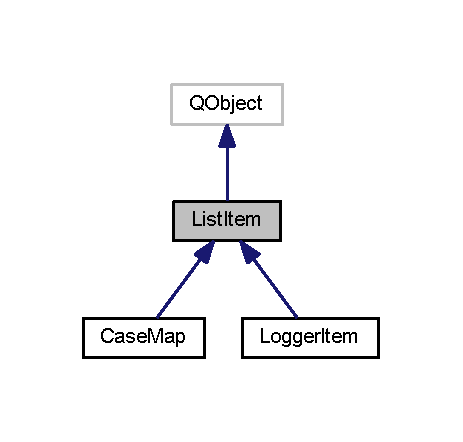
\includegraphics[width=222pt]{class_list_item__inherit__graph}
\end{center}
\end{figure}


Graphe de collaboration de List\+Item\+:
\nopagebreak
\begin{figure}[H]
\begin{center}
\leavevmode
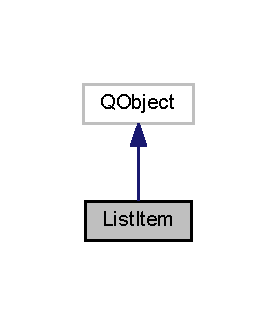
\includegraphics[width=133pt]{class_list_item__coll__graph}
\end{center}
\end{figure}
\subsection*{Signaux}
\begin{DoxyCompactItemize}
\item 
void {\bfseries data\+Changed} ()\hypertarget{class_list_item_a9662031ae22971e1a4d54d85e5911a41}{}\label{class_list_item_a9662031ae22971e1a4d54d85e5911a41}

\end{DoxyCompactItemize}
\subsection*{Fonctions membres publiques}
\begin{DoxyCompactItemize}
\item 
{\bfseries List\+Item} (Q\+Object $\ast$parent=0)\hypertarget{class_list_item_af22aad420e541c1b2ba1bb52e19923fb}{}\label{class_list_item_af22aad420e541c1b2ba1bb52e19923fb}

\item 
virtual Q\+String {\bfseries id} () const  =0\hypertarget{class_list_item_a2bd93b8512b15679bc70d0025458c71c}{}\label{class_list_item_a2bd93b8512b15679bc70d0025458c71c}

\item 
virtual Q\+Variant {\bfseries data} (int role) const  =0\hypertarget{class_list_item_a42655a12963c9fb0f8f80d524d6cafe3}{}\label{class_list_item_a42655a12963c9fb0f8f80d524d6cafe3}

\item 
virtual Q\+Hash$<$ int, Q\+Byte\+Array $>$ {\bfseries role\+Names} () const  =0\hypertarget{class_list_item_a104f771dd730c5f03aa8aa9107eb2e49}{}\label{class_list_item_a104f771dd730c5f03aa8aa9107eb2e49}

\item 
virtual bool {\bfseries set\+Data} (const Q\+Variant \&value, int role)=0\hypertarget{class_list_item_a1f474dc347b3380d5737ee593d5478f0}{}\label{class_list_item_a1f474dc347b3380d5737ee593d5478f0}

\end{DoxyCompactItemize}


La documentation de cette classe a été générée à partir du fichier suivant \+:\begin{DoxyCompactItemize}
\item 
src/\+Map/case\+Map.\+h\end{DoxyCompactItemize}

\hypertarget{class_logger}{}\section{Référence de la classe Logger}
\label{class_logger}\index{Logger@{Logger}}


Graphe d\textquotesingle{}héritage de Logger\+:
\nopagebreak
\begin{figure}[H]
\begin{center}
\leavevmode
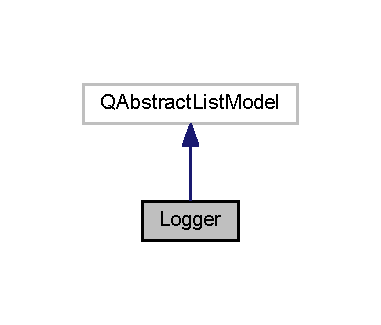
\includegraphics[width=183pt]{class_logger__inherit__graph}
\end{center}
\end{figure}


Graphe de collaboration de Logger\+:
\nopagebreak
\begin{figure}[H]
\begin{center}
\leavevmode
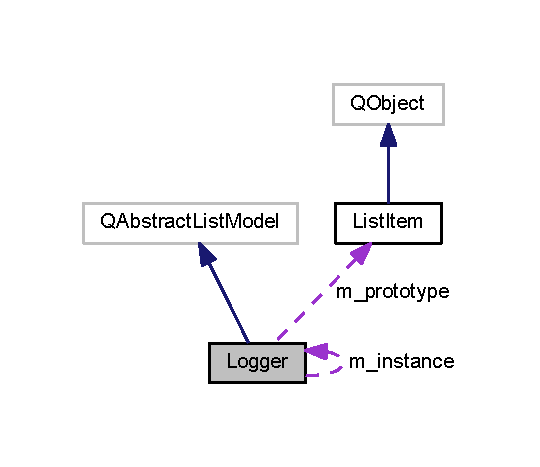
\includegraphics[width=259pt]{class_logger__coll__graph}
\end{center}
\end{figure}
\subsection*{Fonctions membres publiques}
\begin{DoxyCompactItemize}
\item 
int {\bfseries row\+Count} (const Q\+Model\+Index \&parent=Q\+Model\+Index()) const \hypertarget{class_logger_a18c49d472888e90cf665bf94a05e7f7b}{}\label{class_logger_a18c49d472888e90cf665bf94a05e7f7b}

\item 
Q\+Variant {\bfseries data} (const Q\+Model\+Index \&index, int role=Qt\+::\+Display\+Role) const \hypertarget{class_logger_ae958be03d479d1cd0f8965844dddb741}{}\label{class_logger_ae958be03d479d1cd0f8965844dddb741}

\item 
void {\bfseries append\+Row} (\hyperlink{class_list_item}{List\+Item} $\ast$item)\hypertarget{class_logger_a6e93ce928f16dd70a97253a009e680a4}{}\label{class_logger_a6e93ce928f16dd70a97253a009e680a4}

\item 
void {\bfseries append\+Rows} (const Q\+List$<$ \hyperlink{class_list_item}{List\+Item} $\ast$ $>$ \&items)\hypertarget{class_logger_addccef2b72456c7d6183f8b3a3afba25}{}\label{class_logger_addccef2b72456c7d6183f8b3a3afba25}

\item 
Q\+Hash$<$ int, Q\+Byte\+Array $>$ {\bfseries role\+Names} () const \hypertarget{class_logger_ae8e97121859692993d50e9465a3f5db6}{}\label{class_logger_ae8e97121859692993d50e9465a3f5db6}

\item 
void {\bfseries ajouter\+Message} (Q\+String message, Q\+String couleur=\char`\"{}black\char`\"{})\hypertarget{class_logger_aedcf172c2590410f42225de83bf39bf9}{}\label{class_logger_aedcf172c2590410f42225de83bf39bf9}

\item 
void {\bfseries clean} ()\hypertarget{class_logger_a2aabe28b224b55fbf6d7432785cf6d2e}{}\label{class_logger_a2aabe28b224b55fbf6d7432785cf6d2e}

\end{DoxyCompactItemize}
\subsection*{Fonctions membres publiques statiques}
\begin{DoxyCompactItemize}
\item 
static \hyperlink{class_logger}{Logger} $\ast$ {\bfseries get\+Instance} ()\hypertarget{class_logger_afec28ae6d7bdf8f6a0734cb20756de10}{}\label{class_logger_afec28ae6d7bdf8f6a0734cb20756de10}

\end{DoxyCompactItemize}
\subsection*{Fonctions membres protégées}
\begin{DoxyCompactItemize}
\item 
{\bfseries Logger} (Q\+Object $\ast$parent=0)\hypertarget{class_logger_afa8685bc11b59b44d84798e867017e54}{}\label{class_logger_afa8685bc11b59b44d84798e867017e54}

\end{DoxyCompactItemize}
\subsection*{Attributs protégés}
\begin{DoxyCompactItemize}
\item 
\hyperlink{class_list_item}{List\+Item} $\ast$ {\bfseries m\+\_\+prototype}\hypertarget{class_logger_a91a11de410204a2fd0f7d29b88e19297}{}\label{class_logger_a91a11de410204a2fd0f7d29b88e19297}

\item 
Q\+List$<$ \hyperlink{class_list_item}{List\+Item} $\ast$ $>$ {\bfseries m\+\_\+list}\hypertarget{class_logger_a96dc285b52543b6773c6f1d44eb1cb0e}{}\label{class_logger_a96dc285b52543b6773c6f1d44eb1cb0e}

\end{DoxyCompactItemize}
\subsection*{Attributs protégés statiques}
\begin{DoxyCompactItemize}
\item 
static \hyperlink{class_logger}{Logger} $\ast$ {\bfseries m\+\_\+instance} = new \hyperlink{class_logger}{Logger}\hypertarget{class_logger_a59ca6bf951da7c541d9aac5024062690}{}\label{class_logger_a59ca6bf951da7c541d9aac5024062690}

\end{DoxyCompactItemize}


La documentation de cette classe a été générée à partir des fichiers suivants \+:\begin{DoxyCompactItemize}
\item 
src/\+Global/logger.\+h\item 
src/\+Global/logger.\+cpp\end{DoxyCompactItemize}

\hypertarget{class_logger_item}{}\section{Référence de la classe Logger\+Item}
\label{class_logger_item}\index{Logger\+Item@{Logger\+Item}}


Graphe d\textquotesingle{}héritage de Logger\+Item\+:
\nopagebreak
\begin{figure}[H]
\begin{center}
\leavevmode
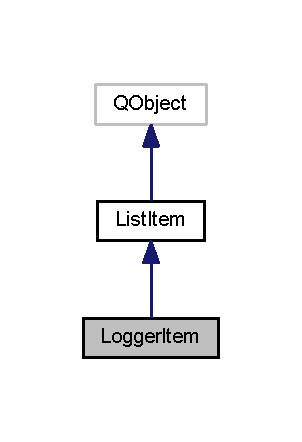
\includegraphics[width=145pt]{class_logger_item__inherit__graph}
\end{center}
\end{figure}


Graphe de collaboration de Logger\+Item\+:
\nopagebreak
\begin{figure}[H]
\begin{center}
\leavevmode
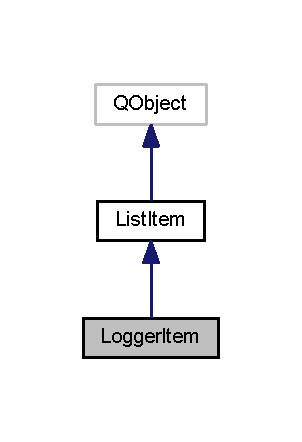
\includegraphics[width=145pt]{class_logger_item__coll__graph}
\end{center}
\end{figure}
\subsection*{Types publics}
\begin{DoxyCompactItemize}
\item 
enum {\bfseries Roles} \{ {\bfseries Date\+Role} = Qt\+:\+:User\+Role+1, 
{\bfseries Message\+Role}, 
{\bfseries Couleur\+Role}
 \}\hypertarget{class_logger_item_a3716eebdcb8cced946f66d3a28d5cc34}{}\label{class_logger_item_a3716eebdcb8cced946f66d3a28d5cc34}

\end{DoxyCompactItemize}
\subsection*{Fonctions membres publiques}
\begin{DoxyCompactItemize}
\item 
{\bfseries Logger\+Item} (Q\+Object $\ast$parent=0)\hypertarget{class_logger_item_ada622893bd2c38aa2b2944ed2d141b00}{}\label{class_logger_item_ada622893bd2c38aa2b2944ed2d141b00}

\item 
{\bfseries Logger\+Item} (Q\+String message, Q\+String couleur, Q\+Object $\ast$parent=0)\hypertarget{class_logger_item_ab309a32922f728dcf2bd4ec732389e75}{}\label{class_logger_item_ab309a32922f728dcf2bd4ec732389e75}

\item 
Q\+Variant {\bfseries data} (int role) const \hypertarget{class_logger_item_a767a5c9088ad19094fefdba8610ded21}{}\label{class_logger_item_a767a5c9088ad19094fefdba8610ded21}

\item 
Q\+Hash$<$ int, Q\+Byte\+Array $>$ {\bfseries role\+Names} () const \hypertarget{class_logger_item_a6f4ef07c47dc7eef231cae42b6c3769b}{}\label{class_logger_item_a6f4ef07c47dc7eef231cae42b6c3769b}

\item 
virtual bool {\bfseries set\+Data} (const Q\+Variant \&value, int role)\hypertarget{class_logger_item_a8cd7bab29e0a08cbb076c4f963d3ed47}{}\label{class_logger_item_a8cd7bab29e0a08cbb076c4f963d3ed47}

\item 
Q\+String {\bfseries id} () const \hypertarget{class_logger_item_ac468e59817754ab6809fa555317ad3d6}{}\label{class_logger_item_ac468e59817754ab6809fa555317ad3d6}

\item 
Q\+String {\bfseries message} () const \hypertarget{class_logger_item_acfc80bd56ae12b8792e529c175aa4072}{}\label{class_logger_item_acfc80bd56ae12b8792e529c175aa4072}

\item 
Q\+String {\bfseries date} () const \hypertarget{class_logger_item_a9421782b0d913cd2b5d7f0b467b670df}{}\label{class_logger_item_a9421782b0d913cd2b5d7f0b467b670df}

\item 
Q\+String {\bfseries couleur} () const \hypertarget{class_logger_item_aebb12082d712174abce71ae97015884b}{}\label{class_logger_item_aebb12082d712174abce71ae97015884b}

\end{DoxyCompactItemize}
\subsection*{Membres hérités additionnels}


La documentation de cette classe a été générée à partir des fichiers suivants \+:\begin{DoxyCompactItemize}
\item 
src/\+Global/logger.\+h\item 
src/\+Global/logger.\+cpp\end{DoxyCompactItemize}

\hypertarget{class_map}{}\section{Référence de la classe Map}
\label{class_map}\index{Map@{Map}}


Graphe d\textquotesingle{}héritage de Map\+:
\nopagebreak
\begin{figure}[H]
\begin{center}
\leavevmode
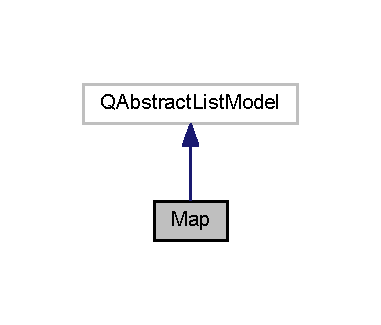
\includegraphics[width=183pt]{class_map__inherit__graph}
\end{center}
\end{figure}


Graphe de collaboration de Map\+:
\nopagebreak
\begin{figure}[H]
\begin{center}
\leavevmode
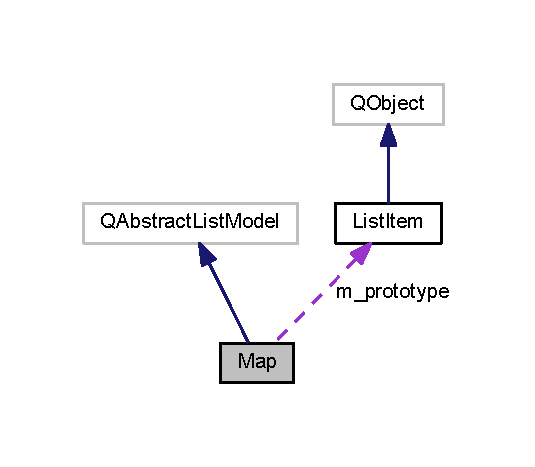
\includegraphics[width=257pt]{class_map__coll__graph}
\end{center}
\end{figure}
\subsection*{Connecteurs publics}
\begin{DoxyCompactItemize}
\item 
Q\+\_\+\+I\+N\+V\+O\+K\+A\+B\+LE int {\bfseries taille\+Case} (int width, int height)\hypertarget{class_map_adfce28a7d4767783e1b7799e5bf6b52e}{}\label{class_map_adfce28a7d4767783e1b7799e5bf6b52e}

\item 
Q\+\_\+\+I\+N\+V\+O\+K\+A\+B\+LE void {\bfseries modifier\+Couleur} (const int row, const Q\+String \&couleur)\hypertarget{class_map_a300d7c1c06a76869fc42beeabcc22484}{}\label{class_map_a300d7c1c06a76869fc42beeabcc22484}

\item 
Q\+\_\+\+I\+N\+V\+O\+K\+A\+B\+LE void {\bfseries modifier\+Position\+Case} (const int row, int x, int y)\hypertarget{class_map_a55963c26007f1414023a058d10748221}{}\label{class_map_a55963c26007f1414023a058d10748221}

\item 
void {\bfseries handle\+Item\+Change} ()\hypertarget{class_map_a7d2fbfcebc184bd902939ea55a40b5de}{}\label{class_map_a7d2fbfcebc184bd902939ea55a40b5de}

\end{DoxyCompactItemize}
\subsection*{Fonctions membres publiques}
\begin{DoxyCompactItemize}
\item 
{\bfseries Map} (Q\+Point dimension, Q\+Object $\ast$parent=0)\hypertarget{class_map_a90ec6843da03a0a35b5bada4505a4635}{}\label{class_map_a90ec6843da03a0a35b5bada4505a4635}

\item 
int {\bfseries row\+Count} (const Q\+Model\+Index \&parent=Q\+Model\+Index()) const \hypertarget{class_map_a862e43cd326ff8b128b975c6baf67299}{}\label{class_map_a862e43cd326ff8b128b975c6baf67299}

\item 
Q\+Variant {\bfseries data} (const Q\+Model\+Index \&index, int role=Qt\+::\+Display\+Role) const \hypertarget{class_map_a75ef3a8e891399024c999c0fbc776fc6}{}\label{class_map_a75ef3a8e891399024c999c0fbc776fc6}

\item 
void {\bfseries append\+Row} (\hyperlink{class_list_item}{List\+Item} $\ast$item)\hypertarget{class_map_af9c1c309f6f8342664501ad584ebccaf}{}\label{class_map_af9c1c309f6f8342664501ad584ebccaf}

\item 
void {\bfseries append\+Rows} (const Q\+List$<$ \hyperlink{class_list_item}{List\+Item} $\ast$ $>$ \&items)\hypertarget{class_map_a1d680ec74568ec6e90c7d6e044e4a489}{}\label{class_map_a1d680ec74568ec6e90c7d6e044e4a489}

\item 
Q\+Hash$<$ int, Q\+Byte\+Array $>$ {\bfseries role\+Names} () const \hypertarget{class_map_af1ec969f88b85d1c90095745cfc599ef}{}\label{class_map_af1ec969f88b85d1c90095745cfc599ef}

\item 
Qt\+::\+Item\+Flags {\bfseries flags} (const Q\+Model\+Index \&index) const \hypertarget{class_map_ac4ce2a5b33e908b860cdf370013c4e9e}{}\label{class_map_ac4ce2a5b33e908b860cdf370013c4e9e}

\item 
bool {\bfseries set\+Data} (const Q\+Model\+Index \&index, const Q\+Variant \&value, int role=Qt\+::\+Edit\+Role)\hypertarget{class_map_a574e69dc23fb4d1a1608d9c9cd120ba6}{}\label{class_map_a574e69dc23fb4d1a1608d9c9cd120ba6}

\item 
Q\+Model\+Index {\bfseries index\+From\+Row} (const int row) const \hypertarget{class_map_a85abd5d3107771ec4137ca8fdf26c12d}{}\label{class_map_a85abd5d3107771ec4137ca8fdf26c12d}

\item 
Q\+Model\+Index {\bfseries index\+From\+Item} (const \hyperlink{class_list_item}{List\+Item} $\ast$item) const \hypertarget{class_map_adae15160f37ac4a09801fd15796d1e57}{}\label{class_map_adae15160f37ac4a09801fd15796d1e57}

\item 
const Q\+Point {\bfseries get\+Dimension} () const \hypertarget{class_map_acb765f109d081944a6306353887f6dcb}{}\label{class_map_acb765f109d081944a6306353887f6dcb}

\item 
int {\bfseries get\+Numero\+Case} (int x, int y) const \hypertarget{class_map_a2804b547704936362ffe8524b5cf4660}{}\label{class_map_a2804b547704936362ffe8524b5cf4660}

\item 
Q\+Point {\bfseries numero\+To\+Point} (int row) const \hypertarget{class_map_a2332ec063b663fb4e7538d9ba8710fb9}{}\label{class_map_a2332ec063b663fb4e7538d9ba8710fb9}

\item 
int {\bfseries get\+Position\+X\+Case} (const int row) const \hypertarget{class_map_aae779485d40677d883c78519f03cc201}{}\label{class_map_aae779485d40677d883c78519f03cc201}

\item 
int {\bfseries get\+Position\+Y\+Case} (const int row) const \hypertarget{class_map_aeb554e4ad8cfd88fbccc852fe053cceb}{}\label{class_map_aeb554e4ad8cfd88fbccc852fe053cceb}

\end{DoxyCompactItemize}
\subsection*{Attributs protégés}
\begin{DoxyCompactItemize}
\item 
int {\bfseries m\+\_\+nombre\+CaseX} = 10\hypertarget{class_map_aa98f997bd04845e62939393f5bda5d15}{}\label{class_map_aa98f997bd04845e62939393f5bda5d15}

\item 
int {\bfseries m\+\_\+nombre\+CaseY} = 10\hypertarget{class_map_a4210d7c188fe60b5d11397ed3b15f09f}{}\label{class_map_a4210d7c188fe60b5d11397ed3b15f09f}

\item 
\hyperlink{class_list_item}{List\+Item} $\ast$ {\bfseries m\+\_\+prototype}\hypertarget{class_map_a86942d2fe84df1a8bf328d0003e3c8e2}{}\label{class_map_a86942d2fe84df1a8bf328d0003e3c8e2}

\item 
Q\+List$<$ \hyperlink{class_list_item}{List\+Item} $\ast$ $>$ {\bfseries m\+\_\+list}\hypertarget{class_map_a7cb44ec468ecd634f6a6390664a596e7}{}\label{class_map_a7cb44ec468ecd634f6a6390664a596e7}

\end{DoxyCompactItemize}


La documentation de cette classe a été générée à partir des fichiers suivants \+:\begin{DoxyCompactItemize}
\item 
src/\+Map/map.\+h\item 
src/\+Map/map.\+cpp\end{DoxyCompactItemize}

\hypertarget{class_moyen}{}\section{Référence de la classe Moyen}
\label{class_moyen}\index{Moyen@{Moyen}}


Graphe d\textquotesingle{}héritage de Moyen\+:
\nopagebreak
\begin{figure}[H]
\begin{center}
\leavevmode
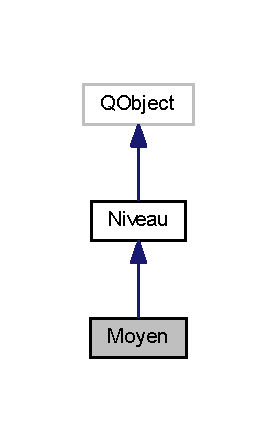
\includegraphics[width=133pt]{class_moyen__inherit__graph}
\end{center}
\end{figure}


Graphe de collaboration de Moyen\+:
\nopagebreak
\begin{figure}[H]
\begin{center}
\leavevmode
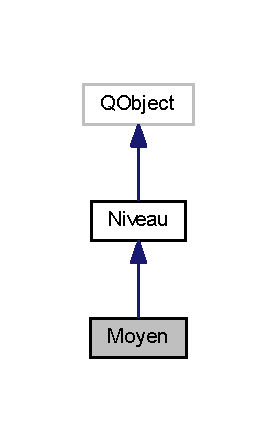
\includegraphics[width=133pt]{class_moyen__coll__graph}
\end{center}
\end{figure}
\subsection*{Fonctions membres publiques}
\begin{DoxyCompactItemize}
\item 
{\bfseries Moyen} (Q\+Object $\ast$parent=0)\hypertarget{class_moyen_aecc34019bec885b6efa891eb00be0734}{}\label{class_moyen_aecc34019bec885b6efa891eb00be0734}

\item 
virtual int {\bfseries resistance\+Navire\+Ordi} ()\hypertarget{class_moyen_a684286278fba33c6274c95b441c1ae86}{}\label{class_moyen_a684286278fba33c6274c95b441c1ae86}

\item 
virtual int {\bfseries resistance\+Navire\+Joueur} ()\hypertarget{class_moyen_af382993bc71204e798501b1e3fe33aa2}{}\label{class_moyen_af382993bc71204e798501b1e3fe33aa2}

\end{DoxyCompactItemize}
\subsection*{Membres hérités additionnels}


La documentation de cette classe a été générée à partir des fichiers suivants \+:\begin{DoxyCompactItemize}
\item 
src/niveau/moyen.\+h\item 
src/niveau/moyen.\+cpp\end{DoxyCompactItemize}

\hypertarget{class_navire}{}\section{Référence de la classe Navire}
\label{class_navire}\index{Navire@{Navire}}


Graphe d\textquotesingle{}héritage de Navire\+:
\nopagebreak
\begin{figure}[H]
\begin{center}
\leavevmode
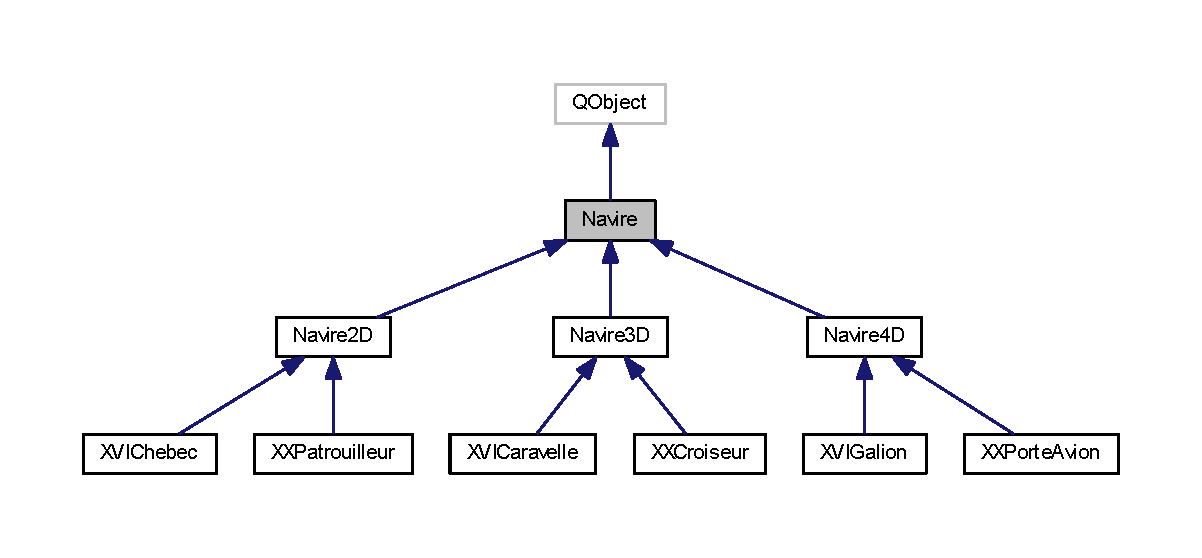
\includegraphics[width=350pt]{class_navire__inherit__graph}
\end{center}
\end{figure}


Graphe de collaboration de Navire\+:
\nopagebreak
\begin{figure}[H]
\begin{center}
\leavevmode
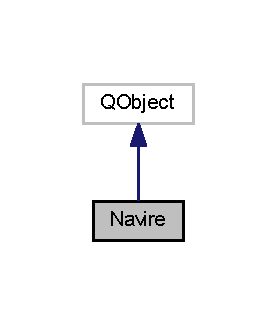
\includegraphics[width=133pt]{class_navire__coll__graph}
\end{center}
\end{figure}
\subsection*{Connecteurs publics}
\begin{DoxyCompactItemize}
\item 
Q\+String {\bfseries image} ()\hypertarget{class_navire_a2af893fa2ff75b29f5fd1a1a916080cd}{}\label{class_navire_a2af893fa2ff75b29f5fd1a1a916080cd}

\end{DoxyCompactItemize}
\subsection*{Signaux}
\begin{DoxyCompactItemize}
\item 
void {\bfseries durabilite\+Changed} ()\hypertarget{class_navire_af6001492dec19fdc15ed08cd99b26ca6}{}\label{class_navire_af6001492dec19fdc15ed08cd99b26ca6}

\end{DoxyCompactItemize}
\subsection*{Fonctions membres publiques}
\begin{DoxyCompactItemize}
\item 
{\bfseries Navire} (int resistance\+Navire, int taille, Q\+String image, Q\+Object $\ast$parent=0)\hypertarget{class_navire_a7592aa386e7cdb2191e6371d864fe906}{}\label{class_navire_a7592aa386e7cdb2191e6371d864fe906}

\item 
virtual Q\+String {\bfseries get\+Fond} () const  =0\hypertarget{class_navire_aa62e28f2704afe3746ade20d709b501b}{}\label{class_navire_aa62e28f2704afe3746ade20d709b501b}

\item 
virtual Q\+String {\bfseries get\+Nom} () const  =0\hypertarget{class_navire_a56df9386755c950a090a88d1fb489c8a}{}\label{class_navire_a56df9386755c950a090a88d1fb489c8a}

\item 
int {\bfseries get\+Taille} ()\hypertarget{class_navire_a95c9ca9886dca33712784b90552e7fbc}{}\label{class_navire_a95c9ca9886dca33712784b90552e7fbc}

\item 
bool {\bfseries est\+Horizontale} ()\hypertarget{class_navire_a0177c715444d6bbb9106ee2cf3f01f4c}{}\label{class_navire_a0177c715444d6bbb9106ee2cf3f01f4c}

\item 
void {\bfseries set\+Horizontale} (bool e)\hypertarget{class_navire_a1b99e6f77f4f29a5b028e7e20db97774}{}\label{class_navire_a1b99e6f77f4f29a5b028e7e20db97774}

\item 
int {\bfseries get\+Durabilite\+At} (int i)\hypertarget{class_navire_aa249b069cccc930a5ad70d98c4d163f6}{}\label{class_navire_aa249b069cccc930a5ad70d98c4d163f6}

\item 
bool {\bfseries set\+Durabilite\+At} (int i)\hypertarget{class_navire_acea86f1c993f4c6e334c20770936c83d}{}\label{class_navire_acea86f1c993f4c6e334c20770936c83d}

\item 
int {\bfseries get\+Max\+Durabilite} ()\hypertarget{class_navire_af84c7380003b15256c703e455842661c}{}\label{class_navire_af84c7380003b15256c703e455842661c}

\item 
bool {\bfseries est\+Detruit} ()\hypertarget{class_navire_a6db2583256f6042cedb86aa8f08c938b}{}\label{class_navire_a6db2583256f6042cedb86aa8f08c938b}

\end{DoxyCompactItemize}
\subsection*{Attributs protégés}
\begin{DoxyCompactItemize}
\item 
int {\bfseries m\+\_\+taille}\hypertarget{class_navire_a208c375a82e7470faa5f945d437e3997}{}\label{class_navire_a208c375a82e7470faa5f945d437e3997}

\item 
bool {\bfseries m\+\_\+horizontale}\hypertarget{class_navire_a9ab74f347ff2c82c93e9fe23dedeb535}{}\label{class_navire_a9ab74f347ff2c82c93e9fe23dedeb535}

\item 
Q\+String {\bfseries m\+\_\+image}\hypertarget{class_navire_a59dadd821c3d7d6704207e8bba2b727c}{}\label{class_navire_a59dadd821c3d7d6704207e8bba2b727c}

\item 
Q\+Vector$<$ int $>$ {\bfseries m\+\_\+durabilite}\hypertarget{class_navire_ac55a7c362a463586f19fd829dd49b49c}{}\label{class_navire_ac55a7c362a463586f19fd829dd49b49c}

\end{DoxyCompactItemize}
\subsection*{Propriétés}
\begin{DoxyCompactItemize}
\item 
int {\bfseries taille}\hypertarget{class_navire_a71cc2dbc39ff07887bbd806f69779411}{}\label{class_navire_a71cc2dbc39ff07887bbd806f69779411}

\item 
bool {\bfseries horizontale}\hypertarget{class_navire_a4d4cbbde75bbd7446634b17a3165d833}{}\label{class_navire_a4d4cbbde75bbd7446634b17a3165d833}

\item 
Q\+String {\bfseries image\+Navire}\hypertarget{class_navire_a27d860bfbc5a4a1c7b4679c8ba008eda}{}\label{class_navire_a27d860bfbc5a4a1c7b4679c8ba008eda}

\end{DoxyCompactItemize}


La documentation de cette classe a été générée à partir des fichiers suivants \+:\begin{DoxyCompactItemize}
\item 
src/\+Global/\+Navire/navire.\+h\item 
src/\+Global/\+Navire/navire.\+cpp\end{DoxyCompactItemize}

\hypertarget{class_navire2_d}{}\section{Référence de la classe Navire2D}
\label{class_navire2_d}\index{Navire2D@{Navire2D}}


Graphe d\textquotesingle{}héritage de Navire2D\+:
\nopagebreak
\begin{figure}[H]
\begin{center}
\leavevmode
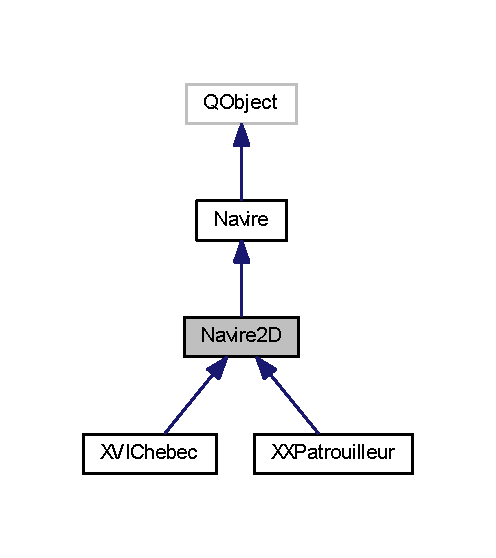
\includegraphics[width=238pt]{class_navire2_d__inherit__graph}
\end{center}
\end{figure}


Graphe de collaboration de Navire2D\+:
\nopagebreak
\begin{figure}[H]
\begin{center}
\leavevmode
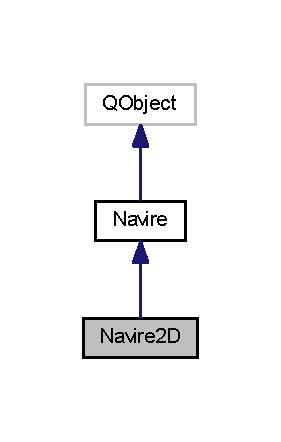
\includegraphics[width=135pt]{class_navire2_d__coll__graph}
\end{center}
\end{figure}
\subsection*{Fonctions membres publiques}
\begin{DoxyCompactItemize}
\item 
{\bfseries Navire2D} (int resistance\+Navire, Q\+String image)\hypertarget{class_navire2_d_a7df7551c7b0833c6d78303347e371c46}{}\label{class_navire2_d_a7df7551c7b0833c6d78303347e371c46}

\item 
virtual Q\+String {\bfseries get\+Fond} () const  =0\hypertarget{class_navire2_d_a9c296afbbff06abc2f6caded7e2f8559}{}\label{class_navire2_d_a9c296afbbff06abc2f6caded7e2f8559}

\end{DoxyCompactItemize}
\subsection*{Membres hérités additionnels}


La documentation de cette classe a été générée à partir des fichiers suivants \+:\begin{DoxyCompactItemize}
\item 
src/\+Global/\+Navire/navire2d.\+h\item 
src/\+Global/\+Navire/navire2d.\+cpp\end{DoxyCompactItemize}

\hypertarget{class_navire3_d}{}\section{Référence de la classe Navire3D}
\label{class_navire3_d}\index{Navire3D@{Navire3D}}


Graphe d\textquotesingle{}héritage de Navire3D\+:
\nopagebreak
\begin{figure}[H]
\begin{center}
\leavevmode
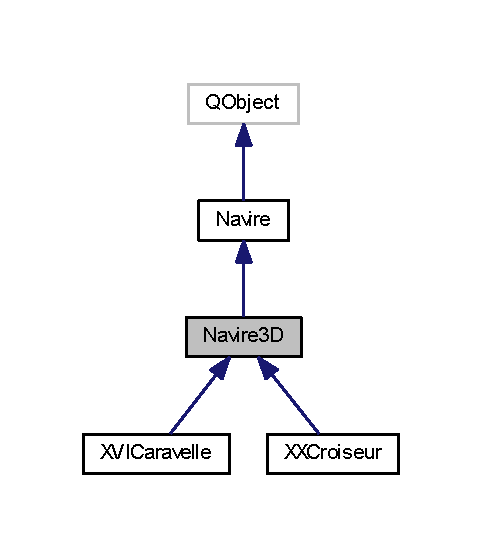
\includegraphics[width=232pt]{class_navire3_d__inherit__graph}
\end{center}
\end{figure}


Graphe de collaboration de Navire3D\+:
\nopagebreak
\begin{figure}[H]
\begin{center}
\leavevmode
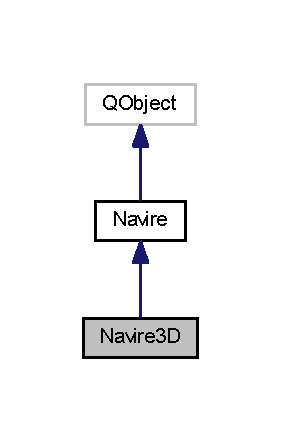
\includegraphics[width=135pt]{class_navire3_d__coll__graph}
\end{center}
\end{figure}
\subsection*{Fonctions membres publiques}
\begin{DoxyCompactItemize}
\item 
{\bfseries Navire3D} (int resistance\+Navire, Q\+String image)\hypertarget{class_navire3_d_aecdf5b49b8220b5d4b91a836b384ed78}{}\label{class_navire3_d_aecdf5b49b8220b5d4b91a836b384ed78}

\item 
virtual Q\+String {\bfseries get\+Fond} () const  =0\hypertarget{class_navire3_d_ae4e5e4d87eebd78b3e08617d45016033}{}\label{class_navire3_d_ae4e5e4d87eebd78b3e08617d45016033}

\end{DoxyCompactItemize}
\subsection*{Membres hérités additionnels}


La documentation de cette classe a été générée à partir des fichiers suivants \+:\begin{DoxyCompactItemize}
\item 
src/\+Global/\+Navire/navire3d.\+h\item 
src/\+Global/\+Navire/navire3d.\+cpp\end{DoxyCompactItemize}

\hypertarget{class_navire4_d}{}\section{Référence de la classe Navire4D}
\label{class_navire4_d}\index{Navire4D@{Navire4D}}


Graphe d\textquotesingle{}héritage de Navire4D\+:
\nopagebreak
\begin{figure}[H]
\begin{center}
\leavevmode
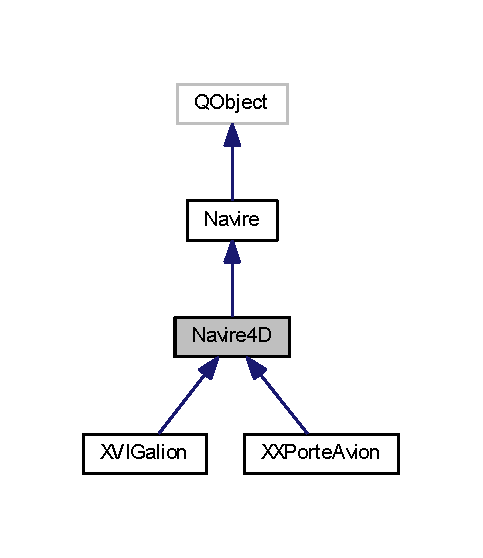
\includegraphics[width=232pt]{class_navire4_d__inherit__graph}
\end{center}
\end{figure}


Graphe de collaboration de Navire4D\+:
\nopagebreak
\begin{figure}[H]
\begin{center}
\leavevmode
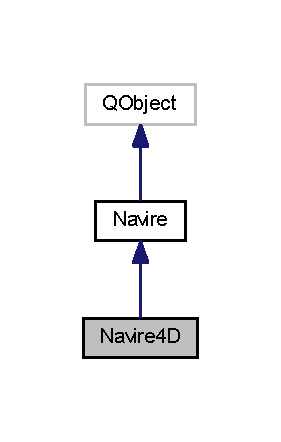
\includegraphics[width=135pt]{class_navire4_d__coll__graph}
\end{center}
\end{figure}
\subsection*{Fonctions membres publiques}
\begin{DoxyCompactItemize}
\item 
{\bfseries Navire4D} (int resistance\+Navire, Q\+String image)\hypertarget{class_navire4_d_a016c727e460ec308ace8dad83413877d}{}\label{class_navire4_d_a016c727e460ec308ace8dad83413877d}

\item 
virtual Q\+String {\bfseries get\+Fond} () const  =0\hypertarget{class_navire4_d_aec41e6cc72972e2f67fd7eb335544538}{}\label{class_navire4_d_aec41e6cc72972e2f67fd7eb335544538}

\end{DoxyCompactItemize}
\subsection*{Membres hérités additionnels}


La documentation de cette classe a été générée à partir des fichiers suivants \+:\begin{DoxyCompactItemize}
\item 
src/\+Global/\+Navire/navire4d.\+h\item 
src/\+Global/\+Navire/navire4d.\+cpp\end{DoxyCompactItemize}

\hypertarget{class_navire_factory}{}\section{Référence de la classe Navire\+Factory}
\label{class_navire_factory}\index{Navire\+Factory@{Navire\+Factory}}


Graphe d\textquotesingle{}héritage de Navire\+Factory\+:
\nopagebreak
\begin{figure}[H]
\begin{center}
\leavevmode
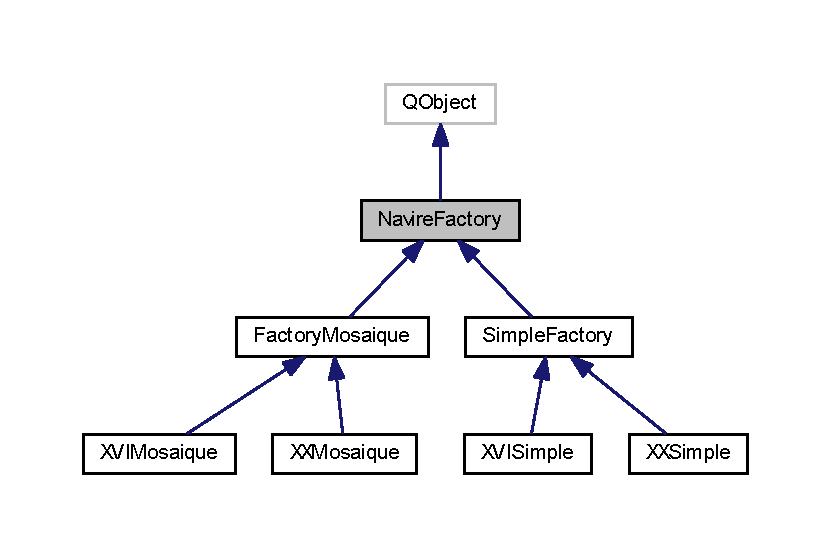
\includegraphics[width=350pt]{class_navire_factory__inherit__graph}
\end{center}
\end{figure}


Graphe de collaboration de Navire\+Factory\+:
\nopagebreak
\begin{figure}[H]
\begin{center}
\leavevmode
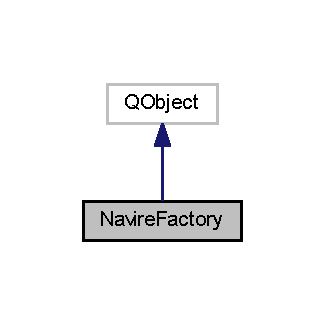
\includegraphics[width=156pt]{class_navire_factory__coll__graph}
\end{center}
\end{figure}
\subsection*{Types publics}
\begin{DoxyCompactItemize}
\item 
enum {\bfseries Type} \{ {\bfseries S\+I\+M\+P\+LE} = 0, 
{\bfseries M\+O\+S\+A\+I\+Q\+UE}
 \}\hypertarget{class_navire_factory_ae1da32b895ef4e65026775e63846729c}{}\label{class_navire_factory_ae1da32b895ef4e65026775e63846729c}

\item 
enum {\bfseries Epoque} \{ {\bfseries X\+VI} =0, 
{\bfseries XX}
 \}\hypertarget{class_navire_factory_a46348deb2727c1f95b2e52cd162151e4}{}\label{class_navire_factory_a46348deb2727c1f95b2e52cd162151e4}

\end{DoxyCompactItemize}
\subsection*{Fonctions membres publiques}
\begin{DoxyCompactItemize}
\item 
{\bfseries Navire\+Factory} (Q\+Object $\ast$parent=0)\hypertarget{class_navire_factory_a7cb54df352b8abca46855b9c2dbbbdff}{}\label{class_navire_factory_a7cb54df352b8abca46855b9c2dbbbdff}

\item 
virtual Q\+List$<$ \hyperlink{class_navire}{Navire} $\ast$ $>$ {\bfseries creer\+Navire} (int nombre, int resistance\+Navire)=0\hypertarget{class_navire_factory_ad663ca3d3fdf6c080c28ce595b55cf21}{}\label{class_navire_factory_ad663ca3d3fdf6c080c28ce595b55cf21}

\end{DoxyCompactItemize}
\subsection*{Fonctions membres publiques statiques}
\begin{DoxyCompactItemize}
\item 
static const Q\+String\+List {\bfseries get\+List\+Type} ()\hypertarget{class_navire_factory_a55100c7a5b9b9c633bb8a7733fbb5f08}{}\label{class_navire_factory_a55100c7a5b9b9c633bb8a7733fbb5f08}

\item 
static const Q\+String\+List {\bfseries get\+List\+Epoque} ()\hypertarget{class_navire_factory_af077dc62c3e994fd7e30e62f3f02029b}{}\label{class_navire_factory_af077dc62c3e994fd7e30e62f3f02029b}

\item 
static Type {\bfseries Stringto\+Type} (Q\+String type)\hypertarget{class_navire_factory_ace4b810b9565550fbab8d5c0a4a690de}{}\label{class_navire_factory_ace4b810b9565550fbab8d5c0a4a690de}

\item 
static Epoque {\bfseries Epoque\+Stringto\+Type} (Q\+String type)\hypertarget{class_navire_factory_a5cc2fc8822fe08fbc120c35fd44d4d0c}{}\label{class_navire_factory_a5cc2fc8822fe08fbc120c35fd44d4d0c}

\end{DoxyCompactItemize}


La documentation de cette classe a été générée à partir des fichiers suivants \+:\begin{DoxyCompactItemize}
\item 
src/\+Global/navire\+Factory/navire\+Factory.\+h\item 
src/\+Global/navire\+Factory/navire\+Factory.\+cpp\end{DoxyCompactItemize}

\hypertarget{class_navire_graphique}{}\section{Référence de la classe Navire\+Graphique}
\label{class_navire_graphique}\index{Navire\+Graphique@{Navire\+Graphique}}


Graphe d\textquotesingle{}héritage de Navire\+Graphique\+:
\nopagebreak
\begin{figure}[H]
\begin{center}
\leavevmode
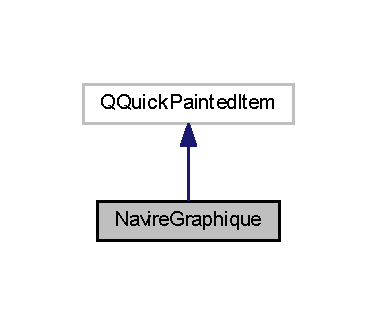
\includegraphics[width=181pt]{class_navire_graphique__inherit__graph}
\end{center}
\end{figure}


Graphe de collaboration de Navire\+Graphique\+:
\nopagebreak
\begin{figure}[H]
\begin{center}
\leavevmode
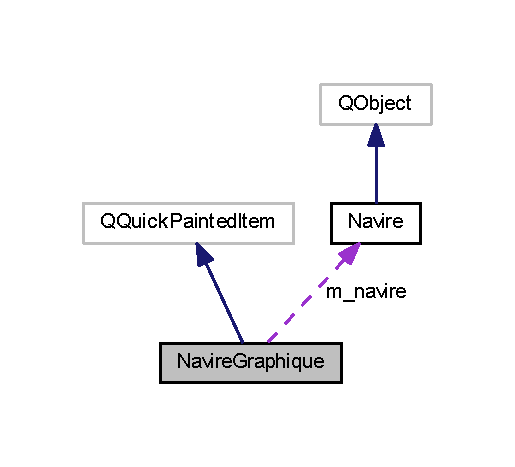
\includegraphics[width=247pt]{class_navire_graphique__coll__graph}
\end{center}
\end{figure}
\subsection*{Connecteurs publics}
\begin{DoxyCompactItemize}
\item 
\hyperlink{class_navire}{Navire} $\ast$ {\bfseries modele} ()\hypertarget{class_navire_graphique_a82f9b5d7e51a400479ed6fb2ae64b001}{}\label{class_navire_graphique_a82f9b5d7e51a400479ed6fb2ae64b001}

\item 
void {\bfseries set\+Modele} (\hyperlink{class_navire}{Navire} $\ast$navire)\hypertarget{class_navire_graphique_aec964f5192f382c794d8bf48d7997aad}{}\label{class_navire_graphique_aec964f5192f382c794d8bf48d7997aad}

\end{DoxyCompactItemize}
\subsection*{Signaux}
\begin{DoxyCompactItemize}
\item 
void {\bfseries modele\+Changed} ()\hypertarget{class_navire_graphique_a8895618937c8cc932ab0cca549574ed0}{}\label{class_navire_graphique_a8895618937c8cc932ab0cca549574ed0}

\end{DoxyCompactItemize}
\subsection*{Fonctions membres publiques}
\begin{DoxyCompactItemize}
\item 
{\bfseries Navire\+Graphique} (Q\+Quick\+Item $\ast$parent=0)\hypertarget{class_navire_graphique_a91106b0259c79f39d6e73fb032c7b879}{}\label{class_navire_graphique_a91106b0259c79f39d6e73fb032c7b879}

\item 
void {\bfseries paint} (Q\+Painter $\ast$painter)\hypertarget{class_navire_graphique_afe5ea560d2957f56a37de9f97b950c68}{}\label{class_navire_graphique_afe5ea560d2957f56a37de9f97b950c68}

\end{DoxyCompactItemize}
\subsection*{Fonctions membres protégées}
\begin{DoxyCompactItemize}
\item 
void {\bfseries dessiner\+Croix} (Q\+Painter $\ast$painter, int x, int y, int w, int h)\hypertarget{class_navire_graphique_a363b5a461391387078fb6126bf41ecc0}{}\label{class_navire_graphique_a363b5a461391387078fb6126bf41ecc0}

\end{DoxyCompactItemize}
\subsection*{Attributs protégés}
\begin{DoxyCompactItemize}
\item 
\hyperlink{class_navire}{Navire} $\ast$ {\bfseries m\+\_\+navire}\hypertarget{class_navire_graphique_abea52cd8d08c1b5a9ceb329c0fec957f}{}\label{class_navire_graphique_abea52cd8d08c1b5a9ceb329c0fec957f}

\end{DoxyCompactItemize}
\subsection*{Propriétés}
\begin{DoxyCompactItemize}
\item 
\hyperlink{class_navire}{Navire} {\bfseries modele}\hypertarget{class_navire_graphique_ad6015761841fe8f6e7d8c72b96d5428e}{}\label{class_navire_graphique_ad6015761841fe8f6e7d8c72b96d5428e}

\end{DoxyCompactItemize}


La documentation de cette classe a été générée à partir des fichiers suivants \+:\begin{DoxyCompactItemize}
\item 
src/\+Graphique/\+Global/\+Navire/naviregraphique.\+h\item 
src/\+Graphique/\+Global/\+Navire/naviregraphique.\+cpp\end{DoxyCompactItemize}

\hypertarget{class_niveau}{}\section{Référence de la classe Niveau}
\label{class_niveau}\index{Niveau@{Niveau}}


Graphe d\textquotesingle{}héritage de Niveau\+:
\nopagebreak
\begin{figure}[H]
\begin{center}
\leavevmode
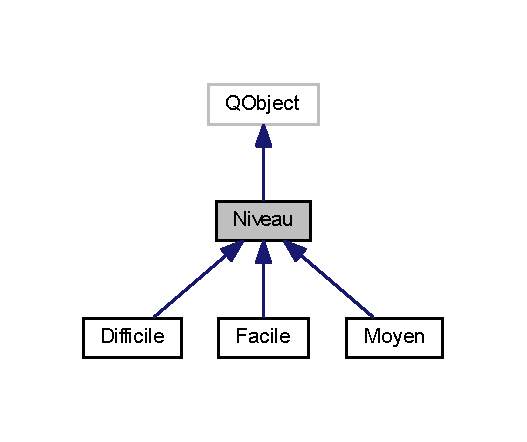
\includegraphics[width=253pt]{class_niveau__inherit__graph}
\end{center}
\end{figure}


Graphe de collaboration de Niveau\+:
\nopagebreak
\begin{figure}[H]
\begin{center}
\leavevmode
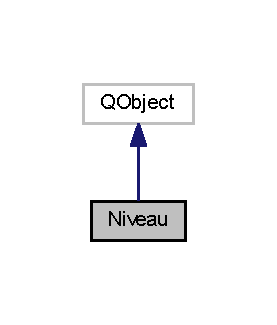
\includegraphics[width=133pt]{class_niveau__coll__graph}
\end{center}
\end{figure}
\subsection*{Connecteurs publics}
\begin{DoxyCompactItemize}
\item 
Q\+String {\bfseries get\+Nom} ()\hypertarget{class_niveau_a3b65ddce29136cdf442b27b6b4e4bc4f}{}\label{class_niveau_a3b65ddce29136cdf442b27b6b4e4bc4f}

\end{DoxyCompactItemize}
\subsection*{Fonctions membres publiques}
\begin{DoxyCompactItemize}
\item 
{\bfseries Niveau} (Q\+String nom, Q\+Object $\ast$parent=0)\hypertarget{class_niveau_a3fbdc4ab93573d004984a3eab293f4d9}{}\label{class_niveau_a3fbdc4ab93573d004984a3eab293f4d9}

\item 
Q\+String {\bfseries afficher} ()\hypertarget{class_niveau_a37e55e6e6c312d586b40835edf84605f}{}\label{class_niveau_a37e55e6e6c312d586b40835edf84605f}

\item 
Q\+String {\bfseries get\+Description} ()\hypertarget{class_niveau_a82ee13fe6015b6ede7d19103fd728cb2}{}\label{class_niveau_a82ee13fe6015b6ede7d19103fd728cb2}

\item 
virtual int {\bfseries resistance\+Navire\+Ordi} ()=0\hypertarget{class_niveau_ad4549b64749f16682e411165ac8c6254}{}\label{class_niveau_ad4549b64749f16682e411165ac8c6254}

\item 
virtual int {\bfseries resistance\+Navire\+Joueur} ()=0\hypertarget{class_niveau_ad42a882c81cfc33d157e18c59accd3cd}{}\label{class_niveau_ad42a882c81cfc33d157e18c59accd3cd}

\end{DoxyCompactItemize}
\subsection*{Attributs protégés}
\begin{DoxyCompactItemize}
\item 
Q\+String {\bfseries m\+\_\+nom}\hypertarget{class_niveau_ae502dc8f2dd3487237d804bb1ea573e5}{}\label{class_niveau_ae502dc8f2dd3487237d804bb1ea573e5}

\end{DoxyCompactItemize}
\subsection*{Propriétés}
\begin{DoxyCompactItemize}
\item 
Q\+String {\bfseries nom}\hypertarget{class_niveau_a422f3ce8febcf42174b60740626b9e6d}{}\label{class_niveau_a422f3ce8febcf42174b60740626b9e6d}

\item 
Q\+String {\bfseries description}\hypertarget{class_niveau_ac77687fe407b44fa85da30bbe9efa41e}{}\label{class_niveau_ac77687fe407b44fa85da30bbe9efa41e}

\end{DoxyCompactItemize}


La documentation de cette classe a été générée à partir des fichiers suivants \+:\begin{DoxyCompactItemize}
\item 
src/niveau/niveau.\+h\item 
src/niveau/niveau.\+cpp\end{DoxyCompactItemize}

\hypertarget{class_partie}{}\section{Référence de la classe Partie}
\label{class_partie}\index{Partie@{Partie}}


Graphe d\textquotesingle{}héritage de Partie\+:
\nopagebreak
\begin{figure}[H]
\begin{center}
\leavevmode
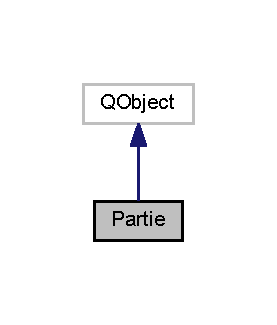
\includegraphics[width=133pt]{class_partie__inherit__graph}
\end{center}
\end{figure}


Graphe de collaboration de Partie\+:
\nopagebreak
\begin{figure}[H]
\begin{center}
\leavevmode
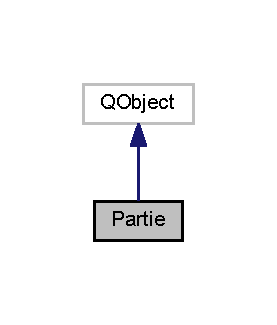
\includegraphics[width=133pt]{class_partie__coll__graph}
\end{center}
\end{figure}
\subsection*{Connecteurs publics}
\begin{DoxyCompactItemize}
\item 
Q\+Variant const {\bfseries get\+Joueur} (int i) const \hypertarget{class_partie_a2901add3c995b28128d69ccad400982c}{}\label{class_partie_a2901add3c995b28128d69ccad400982c}

\end{DoxyCompactItemize}
\subsection*{Signaux}
\begin{DoxyCompactItemize}
\item 
void {\bfseries commencer} (bool placement, int nb\+\_\+navire=0)\hypertarget{class_partie_ad0d567419621d3c7c858a2b005e3e608}{}\label{class_partie_ad0d567419621d3c7c858a2b005e3e608}

\item 
void {\bfseries fin} (Q\+String joueur)\hypertarget{class_partie_a7997238d07a53ad08643b8c280f935db}{}\label{class_partie_a7997238d07a53ad08643b8c280f935db}

\item 
void {\bfseries temps\+Changed} ()\hypertarget{class_partie_a3c9c660c219c59797242aceaaf4ac76c}{}\label{class_partie_a3c9c660c219c59797242aceaaf4ac76c}

\item 
void {\bfseries joueur\+Courant\+Changed} ()\hypertarget{class_partie_a674d35b9052ea2d0a1b63bceea331111}{}\label{class_partie_a674d35b9052ea2d0a1b63bceea331111}

\end{DoxyCompactItemize}
\subsection*{Fonctions membres publiques}
\begin{DoxyCompactItemize}
\item 
{\bfseries Partie} (Q\+Object $\ast$parent=0)\hypertarget{class_partie_a0d540b2932dcd0e53841d7ef079068fa}{}\label{class_partie_a0d540b2932dcd0e53841d7ef079068fa}

\item 
void {\bfseries add\+Joueurs} (\hyperlink{class_joueur}{Joueur} $\ast$j1, \hyperlink{class_joueur}{Joueur} $\ast$j2)\hypertarget{class_partie_a2c87a8323f8b2e90e122027717727e5b}{}\label{class_partie_a2c87a8323f8b2e90e122027717727e5b}

\item 
void {\bfseries set\+Navire\+Factory} (\hyperlink{class_navire_factory}{Navire\+Factory} $\ast$f)\hypertarget{class_partie_a1b37cfa4baa6858c4bcb28de91ebd968}{}\label{class_partie_a1b37cfa4baa6858c4bcb28de91ebd968}

\item 
void \hyperlink{class_partie_afc96e2ca2cc71d244fa5f9b219f10d63}{preparation} (Q\+Point dimension, Q\+String s, bool placement, int nb\+\_\+navire)
\begin{DoxyCompactList}\small\item\em preparation \end{DoxyCompactList}\item 
Q\+\_\+\+I\+N\+V\+O\+K\+A\+B\+LE void \hyperlink{class_partie_a0bb3dd78c418401764f64a047cc865db}{attaquer} (int index\+\_\+joueur, int position)
\begin{DoxyCompactList}\small\item\em \hyperlink{class_partie_a0bb3dd78c418401764f64a047cc865db}{Partie\+::attaquer}. \end{DoxyCompactList}\item 
Q\+\_\+\+I\+N\+V\+O\+K\+A\+B\+LE int {\bfseries nombre\+Joueur} ()\hypertarget{class_partie_a0794b94a8673a8270dfe78c8520d9a7b}{}\label{class_partie_a0794b94a8673a8270dfe78c8520d9a7b}

\item 
Q\+\_\+\+I\+N\+V\+O\+K\+A\+B\+LE Q\+Variant {\bfseries get\+Next\+Joueur\+A\+Placer} ()\hypertarget{class_partie_a9cf5798d985bfb538895057c5a6b650a}{}\label{class_partie_a9cf5798d985bfb538895057c5a6b650a}

\item 
Q\+\_\+\+I\+N\+V\+O\+K\+A\+B\+LE void {\bfseries lancer} ()\hypertarget{class_partie_a932d5700f97a39216697feff60960b1b}{}\label{class_partie_a932d5700f97a39216697feff60960b1b}

\item 
void {\bfseries set\+Strategie} (Q\+String s)\hypertarget{class_partie_a77bcc0a53bd522d2deb957205115ebbf}{}\label{class_partie_a77bcc0a53bd522d2deb957205115ebbf}

\end{DoxyCompactItemize}
\subsection*{Propriétés}
\begin{DoxyCompactItemize}
\item 
int {\bfseries temps}\hypertarget{class_partie_af0505e67137db0a5ce5a64007abcf477}{}\label{class_partie_af0505e67137db0a5ce5a64007abcf477}

\item 
Q\+String {\bfseries joueur\+Courant}\hypertarget{class_partie_a5c3808018f9728a364cdad7457e00ace}{}\label{class_partie_a5c3808018f9728a364cdad7457e00ace}

\end{DoxyCompactItemize}


\subsection{Documentation des fonctions membres}
\index{Partie@{Partie}!attaquer@{attaquer}}
\index{attaquer@{attaquer}!Partie@{Partie}}
\subsubsection[{\texorpdfstring{attaquer(int index\+\_\+joueur, int position)}{attaquer(int index_joueur, int position)}}]{\setlength{\rightskip}{0pt plus 5cm}void Partie\+::attaquer (
\begin{DoxyParamCaption}
\item[{int}]{index\+\_\+joueur, }
\item[{int}]{position}
\end{DoxyParamCaption}
)}\hypertarget{class_partie_a0bb3dd78c418401764f64a047cc865db}{}\label{class_partie_a0bb3dd78c418401764f64a047cc865db}


\hyperlink{class_partie_a0bb3dd78c418401764f64a047cc865db}{Partie\+::attaquer}. 


\begin{DoxyParams}{Paramètres}
{\em index\+\_\+joueur} & numero de position dans la liste des joueurs (joueur qui est attaqué) \\
\hline
{\em position} & case \\
\hline
\end{DoxyParams}
\index{Partie@{Partie}!preparation@{preparation}}
\index{preparation@{preparation}!Partie@{Partie}}
\subsubsection[{\texorpdfstring{preparation(\+Q\+Point dimension, Q\+String s, bool placement, int nb\+\_\+navire)}{preparation(QPoint dimension, QString s, bool placement, int nb_navire)}}]{\setlength{\rightskip}{0pt plus 5cm}void Partie\+::preparation (
\begin{DoxyParamCaption}
\item[{Q\+Point}]{dimension, }
\item[{Q\+String}]{strategie, }
\item[{bool}]{placement, }
\item[{int}]{nb\+\_\+navire}
\end{DoxyParamCaption}
)}\hypertarget{class_partie_afc96e2ca2cc71d244fa5f9b219f10d63}{}\label{class_partie_afc96e2ca2cc71d244fa5f9b219f10d63}


preparation 

Partie\+::start.


\begin{DoxyParams}{Paramètres}
{\em placement} & false placement automatique, true choix du joueur\\
\hline
{\em placement} & true \+: le joueur choisit sa place, false sinon \\
\hline
\end{DoxyParams}


La documentation de cette classe a été générée à partir des fichiers suivants \+:\begin{DoxyCompactItemize}
\item 
src/\+Global/partie.\+h\item 
src/\+Global/partie.\+cpp\end{DoxyCompactItemize}

\hypertarget{class_partie_factory}{}\section{Référence de la classe Partie\+Factory}
\label{class_partie_factory}\index{Partie\+Factory@{Partie\+Factory}}


Graphe d\textquotesingle{}héritage de Partie\+Factory\+:
\nopagebreak
\begin{figure}[H]
\begin{center}
\leavevmode
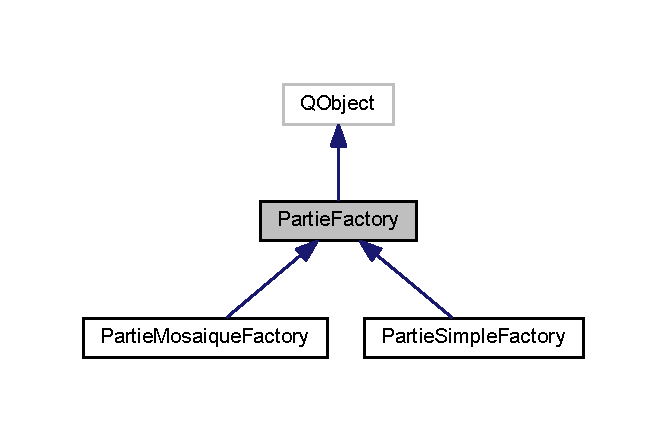
\includegraphics[width=320pt]{class_partie_factory__inherit__graph}
\end{center}
\end{figure}


Graphe de collaboration de Partie\+Factory\+:
\nopagebreak
\begin{figure}[H]
\begin{center}
\leavevmode
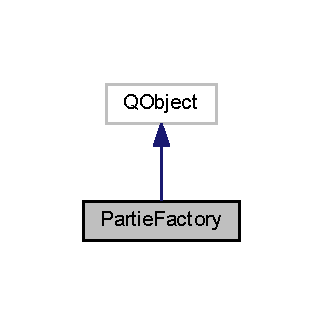
\includegraphics[width=155pt]{class_partie_factory__coll__graph}
\end{center}
\end{figure}
\subsection*{Fonctions membres publiques}
\begin{DoxyCompactItemize}
\item 
{\bfseries Partie\+Factory} (Q\+Object $\ast$parent=0)\hypertarget{class_partie_factory_aa379328311144a9192f3bf662c7c6a3e}{}\label{class_partie_factory_aa379328311144a9192f3bf662c7c6a3e}

\item 
\hyperlink{class_partie}{Partie} $\ast$ {\bfseries creer\+Partie} (Navire\+Factory\+::\+Epoque epoque, int nb\+\_\+navire, \hyperlink{class_niveau}{Niveau} $\ast$niveau)\hypertarget{class_partie_factory_ae6146894dd3dc428122632ad6033d524}{}\label{class_partie_factory_ae6146894dd3dc428122632ad6033d524}

\end{DoxyCompactItemize}
\subsection*{Fonctions membres protégées}
\begin{DoxyCompactItemize}
\item 
virtual \hyperlink{class_navire_factory}{Navire\+Factory} $\ast$ {\bfseries creer\+Navire\+Factory} (Navire\+Factory\+::\+Epoque epoque)=0\hypertarget{class_partie_factory_a4ca8f93c010bfd48cef57e9b2ee7a1a1}{}\label{class_partie_factory_a4ca8f93c010bfd48cef57e9b2ee7a1a1}

\end{DoxyCompactItemize}
\subsection*{Attributs protégés}
\begin{DoxyCompactItemize}
\item 
Q\+Hash$<$ Navire\+Factory\+::\+Epoque, \hyperlink{class_navire_factory}{Navire\+Factory} $\ast$ $>$ {\bfseries m\+\_\+dictionnaire}\hypertarget{class_partie_factory_afe72400900dedead78486633a6ad6b08}{}\label{class_partie_factory_afe72400900dedead78486633a6ad6b08}

\end{DoxyCompactItemize}


La documentation de cette classe a été générée à partir des fichiers suivants \+:\begin{DoxyCompactItemize}
\item 
src/\+Global/partie\+Factory/partiefactory.\+h\item 
src/\+Global/partie\+Factory/partiefactory.\+cpp\end{DoxyCompactItemize}

\hypertarget{class_partie_mosaique_factory}{}\section{Référence de la classe Partie\+Mosaique\+Factory}
\label{class_partie_mosaique_factory}\index{Partie\+Mosaique\+Factory@{Partie\+Mosaique\+Factory}}


Graphe d\textquotesingle{}héritage de Partie\+Mosaique\+Factory\+:
\nopagebreak
\begin{figure}[H]
\begin{center}
\leavevmode
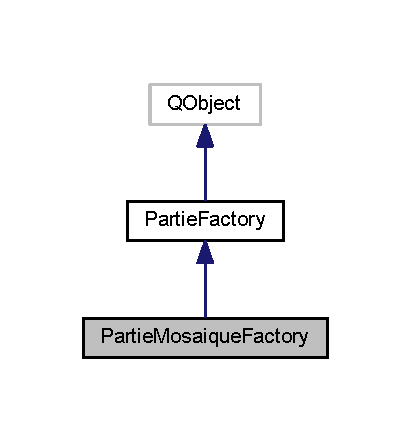
\includegraphics[width=197pt]{class_partie_mosaique_factory__inherit__graph}
\end{center}
\end{figure}


Graphe de collaboration de Partie\+Mosaique\+Factory\+:
\nopagebreak
\begin{figure}[H]
\begin{center}
\leavevmode
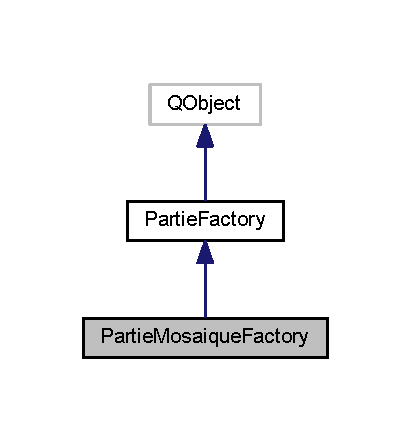
\includegraphics[width=197pt]{class_partie_mosaique_factory__coll__graph}
\end{center}
\end{figure}
\subsection*{Fonctions membres protégées}
\begin{DoxyCompactItemize}
\item 
virtual \hyperlink{class_navire_factory}{Navire\+Factory} $\ast$ {\bfseries creer\+Navire\+Factory} (Navire\+Factory\+::\+Epoque epoque)\hypertarget{class_partie_mosaique_factory_a70ded06da7f02a92db150eafce9e32a1}{}\label{class_partie_mosaique_factory_a70ded06da7f02a92db150eafce9e32a1}

\end{DoxyCompactItemize}
\subsection*{Membres hérités additionnels}


La documentation de cette classe a été générée à partir des fichiers suivants \+:\begin{DoxyCompactItemize}
\item 
src/\+Global/partie\+Factory/partiemosaiqufactory.\+h\item 
src/\+Global/partie\+Factory/partiemosaiqueafactory.\+cpp\end{DoxyCompactItemize}

\hypertarget{class_partie_simple_factory}{}\section{Référence de la classe Partie\+Simple\+Factory}
\label{class_partie_simple_factory}\index{Partie\+Simple\+Factory@{Partie\+Simple\+Factory}}


Graphe d\textquotesingle{}héritage de Partie\+Simple\+Factory\+:
\nopagebreak
\begin{figure}[H]
\begin{center}
\leavevmode
\includegraphics[width=185pt]{class_partie_simple_factory__inherit__graph}
\end{center}
\end{figure}


Graphe de collaboration de Partie\+Simple\+Factory\+:
\nopagebreak
\begin{figure}[H]
\begin{center}
\leavevmode
\includegraphics[width=185pt]{class_partie_simple_factory__coll__graph}
\end{center}
\end{figure}
\subsection*{Fonctions membres protégées}
\begin{DoxyCompactItemize}
\item 
virtual \hyperlink{class_navire_factory}{Navire\+Factory} $\ast$ {\bfseries creer\+Navire\+Factory} (Navire\+Factory\+::\+Epoque epoque)\hypertarget{class_partie_simple_factory_a3598a8b81b8738be235eaa47d1bd8a51}{}\label{class_partie_simple_factory_a3598a8b81b8738be235eaa47d1bd8a51}

\end{DoxyCompactItemize}
\subsection*{Membres hérités additionnels}


La documentation de cette classe a été générée à partir des fichiers suivants \+:\begin{DoxyCompactItemize}
\item 
src/\+Global/partie\+Factory/partiesimplefactory.\+h\item 
src/\+Global/partie\+Factory/partiesimplefactory.\+cpp\end{DoxyCompactItemize}

\hypertarget{struct_joueur_1_1_position}{}\section{Référence de la structure Joueur\+:\+:Position}
\label{struct_joueur_1_1_position}\index{Joueur\+::\+Position@{Joueur\+::\+Position}}
\subsection*{Fonctions membres publiques}
\begin{DoxyCompactItemize}
\item 
bool {\bfseries operator==} (const \hyperlink{struct_joueur_1_1_position}{Position} \&a) const \hypertarget{struct_joueur_1_1_position_a4e5bcfaa0ed20ecf1b9514f307979498}{}\label{struct_joueur_1_1_position_a4e5bcfaa0ed20ecf1b9514f307979498}

\item 
{\bfseries operator Q\+String} () const \hypertarget{struct_joueur_1_1_position_a71fe6feabb1b43d4e99b05e66931999d}{}\label{struct_joueur_1_1_position_a71fe6feabb1b43d4e99b05e66931999d}

\end{DoxyCompactItemize}
\subsection*{Attributs publics}
\begin{DoxyCompactItemize}
\item 
int {\bfseries case\+\_\+id}\hypertarget{struct_joueur_1_1_position_af3f0ac35c0e10cfc1ce7c4c5ab597c58}{}\label{struct_joueur_1_1_position_af3f0ac35c0e10cfc1ce7c4c5ab597c58}

\item 
int {\bfseries bateau\+\_\+partie}\hypertarget{struct_joueur_1_1_position_a56b4777ed97a2ef2a1462a54103e5668}{}\label{struct_joueur_1_1_position_a56b4777ed97a2ef2a1462a54103e5668}

\end{DoxyCompactItemize}


La documentation de cette structure a été générée à partir du fichier suivant \+:\begin{DoxyCompactItemize}
\item 
src/\+Global/joueur.\+h\end{DoxyCompactItemize}

\hypertarget{class_simple_factory}{}\section{Référence de la classe Simple\+Factory}
\label{class_simple_factory}\index{Simple\+Factory@{Simple\+Factory}}


Graphe d\textquotesingle{}héritage de Simple\+Factory\+:
\nopagebreak
\begin{figure}[H]
\begin{center}
\leavevmode
\includegraphics[width=216pt]{class_simple_factory__inherit__graph}
\end{center}
\end{figure}


Graphe de collaboration de Simple\+Factory\+:
\nopagebreak
\begin{figure}[H]
\begin{center}
\leavevmode
\includegraphics[width=160pt]{class_simple_factory__coll__graph}
\end{center}
\end{figure}
\subsection*{Fonctions membres publiques}
\begin{DoxyCompactItemize}
\item 
virtual Q\+List$<$ \hyperlink{class_navire}{Navire} $\ast$ $>$ {\bfseries creer\+Navire} (int nombre, int resistance\+Navire)\hypertarget{class_simple_factory_af2c8730a810a997d360e3aa3d8247d03}{}\label{class_simple_factory_af2c8730a810a997d360e3aa3d8247d03}

\end{DoxyCompactItemize}
\subsection*{Fonctions membres protégées}
\begin{DoxyCompactItemize}
\item 
virtual \hyperlink{class_navire}{Navire} $\ast$ {\bfseries nouveau\+Navire2D} (int resistance\+Navire)=0\hypertarget{class_simple_factory_a80289ea3cc80da52216a4fc2dcd5057b}{}\label{class_simple_factory_a80289ea3cc80da52216a4fc2dcd5057b}

\item 
virtual \hyperlink{class_navire}{Navire} $\ast$ {\bfseries nouveau\+Navire3D} (int resistance\+Navire)=0\hypertarget{class_simple_factory_ad3451c4bf206ebd42c5ac1592fd89607}{}\label{class_simple_factory_ad3451c4bf206ebd42c5ac1592fd89607}

\item 
virtual \hyperlink{class_navire}{Navire} $\ast$ {\bfseries nouveau\+Navire4D} (int resistance\+Navire)=0\hypertarget{class_simple_factory_a86072a6a7828bf45fbb98af88d82a551}{}\label{class_simple_factory_a86072a6a7828bf45fbb98af88d82a551}

\end{DoxyCompactItemize}
\subsection*{Attributs protégés}
\begin{DoxyCompactItemize}
\item 
Q\+Hash$<$ int, \hyperlink{class_navire}{Navire} $\ast$(Simple\+Factory\+::$\ast$)(int)$>$ {\bfseries m\+\_\+dictionnaire}\hypertarget{class_simple_factory_a3bb8cf70370b7b11d8c4c454c2b45645}{}\label{class_simple_factory_a3bb8cf70370b7b11d8c4c454c2b45645}

\item 
int {\bfseries m\+\_\+historique} = -\/1\hypertarget{class_simple_factory_a52e7d40045d933245ac5b88635a818de}{}\label{class_simple_factory_a52e7d40045d933245ac5b88635a818de}

\end{DoxyCompactItemize}
\subsection*{Membres hérités additionnels}


La documentation de cette classe a été générée à partir des fichiers suivants \+:\begin{DoxyCompactItemize}
\item 
src/\+Global/navire\+Factory/simplefactory.\+h\item 
src/\+Global/navire\+Factory/simplefactory.\+cpp\end{DoxyCompactItemize}

\hypertarget{class_strategie_attaque}{}\section{Référence de la classe Strategie\+Attaque}
\label{class_strategie_attaque}\index{Strategie\+Attaque@{Strategie\+Attaque}}


The \hyperlink{class_strategie_attaque}{Strategie\+Attaque} class classe abstraite.  




{\ttfamily \#include $<$strategieattaque.\+h$>$}



Graphe d\textquotesingle{}héritage de Strategie\+Attaque\+:
\nopagebreak
\begin{figure}[H]
\begin{center}
\leavevmode
\includegraphics[width=263pt]{class_strategie_attaque__inherit__graph}
\end{center}
\end{figure}


Graphe de collaboration de Strategie\+Attaque\+:
\nopagebreak
\begin{figure}[H]
\begin{center}
\leavevmode
\includegraphics[width=169pt]{class_strategie_attaque__coll__graph}
\end{center}
\end{figure}
\subsection*{Fonctions membres publiques}
\begin{DoxyCompactItemize}
\item 
{\bfseries Strategie\+Attaque} (Q\+Object $\ast$parent=0)\hypertarget{class_strategie_attaque_a8d01abad58c97da99157439509a773c1}{}\label{class_strategie_attaque_a8d01abad58c97da99157439509a773c1}

\item 
virtual Q\+Point {\bfseries cibler} (const Q\+Vector$<$ Q\+Point $>$ $\ast$coup\+\_\+dispo, const Q\+Point \&map\+\_\+dimension)=0\hypertarget{class_strategie_attaque_a6f1525d085ed45e326833148348b701e}{}\label{class_strategie_attaque_a6f1525d085ed45e326833148348b701e}

\end{DoxyCompactItemize}


\subsection{Description détaillée}
The \hyperlink{class_strategie_attaque}{Strategie\+Attaque} class classe abstraite. 

La documentation de cette classe a été générée à partir des fichiers suivants \+:\begin{DoxyCompactItemize}
\item 
src/strategie/strategieattaque.\+h\item 
src/strategie/strategieattaque.\+cpp\end{DoxyCompactItemize}

\hypertarget{class_theme_manager}{}\section{Référence de la classe Theme\+Manager}
\label{class_theme_manager}\index{Theme\+Manager@{Theme\+Manager}}


Graphe d\textquotesingle{}héritage de Theme\+Manager\+:
\nopagebreak
\begin{figure}[H]
\begin{center}
\leavevmode
\includegraphics[width=163pt]{class_theme_manager__inherit__graph}
\end{center}
\end{figure}


Graphe de collaboration de Theme\+Manager\+:
\nopagebreak
\begin{figure}[H]
\begin{center}
\leavevmode
\includegraphics[width=163pt]{class_theme_manager__coll__graph}
\end{center}
\end{figure}
\subsection*{Connecteurs publics}
\begin{DoxyCompactItemize}
\item 
Q\+String {\bfseries theme} ()\hypertarget{class_theme_manager_accbbfe5ffc08e825f81dbe017fdd8055}{}\label{class_theme_manager_accbbfe5ffc08e825f81dbe017fdd8055}

\item 
void {\bfseries set\+Theme} (Q\+String const \&theme)\hypertarget{class_theme_manager_a5f360969d2cd1fccf3fd204494e262de}{}\label{class_theme_manager_a5f360969d2cd1fccf3fd204494e262de}

\end{DoxyCompactItemize}
\subsection*{Signaux}
\begin{DoxyCompactItemize}
\item 
void {\bfseries theme\+Changed} ()\hypertarget{class_theme_manager_a6e64af50ca5000e922470470d0ca419e}{}\label{class_theme_manager_a6e64af50ca5000e922470470d0ca419e}

\end{DoxyCompactItemize}
\subsection*{Fonctions membres publiques}
\begin{DoxyCompactItemize}
\item 
Q\+Qml\+Engine $\ast$ {\bfseries get\+Engine} ()\hypertarget{class_theme_manager_adf57a1d113b0fe94263a58260aa36317}{}\label{class_theme_manager_adf57a1d113b0fe94263a58260aa36317}

\end{DoxyCompactItemize}
\subsection*{Fonctions membres publiques statiques}
\begin{DoxyCompactItemize}
\item 
static \hyperlink{class_theme_manager}{Theme\+Manager} $\ast$ {\bfseries get\+Instance} (Q\+Qml\+Engine $\ast$engine=nullptr)\hypertarget{class_theme_manager_a657d0bdc7b912e733432fb1cb2ffbc56}{}\label{class_theme_manager_a657d0bdc7b912e733432fb1cb2ffbc56}

\end{DoxyCompactItemize}
\subsection*{Propriétés}
\begin{DoxyCompactItemize}
\item 
Q\+String {\bfseries theme}\hypertarget{class_theme_manager_aef7be23ae1399864a637b130d7c28b27}{}\label{class_theme_manager_aef7be23ae1399864a637b130d7c28b27}

\end{DoxyCompactItemize}


La documentation de cette classe a été générée à partir des fichiers suivants \+:\begin{DoxyCompactItemize}
\item 
src/thememanager.\+h\item 
src/thememanager.\+cpp\end{DoxyCompactItemize}

\hypertarget{class_x_v_i_caravelle}{}\section{Référence de la classe X\+V\+I\+Caravelle}
\label{class_x_v_i_caravelle}\index{X\+V\+I\+Caravelle@{X\+V\+I\+Caravelle}}


Graphe d\textquotesingle{}héritage de X\+V\+I\+Caravelle\+:
\nopagebreak
\begin{figure}[H]
\begin{center}
\leavevmode
\includegraphics[width=150pt]{class_x_v_i_caravelle__inherit__graph}
\end{center}
\end{figure}


Graphe de collaboration de X\+V\+I\+Caravelle\+:
\nopagebreak
\begin{figure}[H]
\begin{center}
\leavevmode
\includegraphics[width=150pt]{class_x_v_i_caravelle__coll__graph}
\end{center}
\end{figure}
\subsection*{Fonctions membres publiques}
\begin{DoxyCompactItemize}
\item 
{\bfseries X\+V\+I\+Caravelle} (int resistance\+Navire)\hypertarget{class_x_v_i_caravelle_a2316f9e79810594371fffe5d0dcb57b3}{}\label{class_x_v_i_caravelle_a2316f9e79810594371fffe5d0dcb57b3}

\item 
virtual Q\+String {\bfseries get\+Fond} () const \hypertarget{class_x_v_i_caravelle_a4c710186bc9a01b541528d12840dc8f1}{}\label{class_x_v_i_caravelle_a4c710186bc9a01b541528d12840dc8f1}

\item 
virtual Q\+String {\bfseries get\+Nom} () const \hypertarget{class_x_v_i_caravelle_af26fba914a34f8eca6191b0d6aebe9fa}{}\label{class_x_v_i_caravelle_af26fba914a34f8eca6191b0d6aebe9fa}

\end{DoxyCompactItemize}
\subsection*{Membres hérités additionnels}


La documentation de cette classe a été générée à partir des fichiers suivants \+:\begin{DoxyCompactItemize}
\item 
src/\+Global/\+Navire/xvicaravelle.\+h\item 
src/\+Global/\+Navire/xvicaravelle.\+cpp\end{DoxyCompactItemize}

\hypertarget{class_x_v_i_chebec}{}\section{Référence de la classe X\+V\+I\+Chebec}
\label{class_x_v_i_chebec}\index{X\+V\+I\+Chebec@{X\+V\+I\+Chebec}}


Graphe d\textquotesingle{}héritage de X\+V\+I\+Chebec\+:
\nopagebreak
\begin{figure}[H]
\begin{center}
\leavevmode
\includegraphics[width=144pt]{class_x_v_i_chebec__inherit__graph}
\end{center}
\end{figure}


Graphe de collaboration de X\+V\+I\+Chebec\+:
\nopagebreak
\begin{figure}[H]
\begin{center}
\leavevmode
\includegraphics[width=144pt]{class_x_v_i_chebec__coll__graph}
\end{center}
\end{figure}
\subsection*{Fonctions membres publiques}
\begin{DoxyCompactItemize}
\item 
{\bfseries X\+V\+I\+Chebec} (int resistance\+Navire)\hypertarget{class_x_v_i_chebec_ae17710ff3c99cd64a25c2559e7f1bc50}{}\label{class_x_v_i_chebec_ae17710ff3c99cd64a25c2559e7f1bc50}

\item 
virtual Q\+String {\bfseries get\+Fond} () const \hypertarget{class_x_v_i_chebec_ad7ee8f1a16832307b56eee644ac71bbd}{}\label{class_x_v_i_chebec_ad7ee8f1a16832307b56eee644ac71bbd}

\item 
virtual Q\+String {\bfseries get\+Nom} () const \hypertarget{class_x_v_i_chebec_a519a55a9fe50c52085423224caed0974}{}\label{class_x_v_i_chebec_a519a55a9fe50c52085423224caed0974}

\end{DoxyCompactItemize}
\subsection*{Membres hérités additionnels}


La documentation de cette classe a été générée à partir des fichiers suivants \+:\begin{DoxyCompactItemize}
\item 
src/\+Global/\+Navire/xvichebec.\+h\item 
src/\+Global/\+Navire/xvichebec.\+cpp\end{DoxyCompactItemize}

\hypertarget{class_x_v_i_galion}{}\section{Référence de la classe X\+V\+I\+Galion}
\label{class_x_v_i_galion}\index{X\+V\+I\+Galion@{X\+V\+I\+Galion}}


Graphe d\textquotesingle{}héritage de X\+V\+I\+Galion\+:
\nopagebreak
\begin{figure}[H]
\begin{center}
\leavevmode
\includegraphics[width=139pt]{class_x_v_i_galion__inherit__graph}
\end{center}
\end{figure}


Graphe de collaboration de X\+V\+I\+Galion\+:
\nopagebreak
\begin{figure}[H]
\begin{center}
\leavevmode
\includegraphics[width=139pt]{class_x_v_i_galion__coll__graph}
\end{center}
\end{figure}
\subsection*{Fonctions membres publiques}
\begin{DoxyCompactItemize}
\item 
{\bfseries X\+V\+I\+Galion} (int resistance\+Navire)\hypertarget{class_x_v_i_galion_a6dc33193c2b8d2696ca4de898712374a}{}\label{class_x_v_i_galion_a6dc33193c2b8d2696ca4de898712374a}

\item 
virtual Q\+String {\bfseries get\+Fond} () const \hypertarget{class_x_v_i_galion_aff1ffbb0603eafdf4343cbafcf001011}{}\label{class_x_v_i_galion_aff1ffbb0603eafdf4343cbafcf001011}

\item 
virtual Q\+String {\bfseries get\+Nom} () const \hypertarget{class_x_v_i_galion_a1df077a9bfee4aed90f489917c9469ff}{}\label{class_x_v_i_galion_a1df077a9bfee4aed90f489917c9469ff}

\end{DoxyCompactItemize}
\subsection*{Membres hérités additionnels}


La documentation de cette classe a été générée à partir des fichiers suivants \+:\begin{DoxyCompactItemize}
\item 
src/\+Global/\+Navire/xvigalion.\+h\item 
src/\+Global/\+Navire/xvigalion.\+cpp\end{DoxyCompactItemize}

\hypertarget{class_x_v_i_mosaique}{}\section{Référence de la classe X\+V\+I\+Mosaique}
\label{class_x_v_i_mosaique}\index{X\+V\+I\+Mosaique@{X\+V\+I\+Mosaique}}


Graphe d\textquotesingle{}héritage de X\+V\+I\+Mosaique\+:
\nopagebreak
\begin{figure}[H]
\begin{center}
\leavevmode
\includegraphics[width=172pt]{class_x_v_i_mosaique__inherit__graph}
\end{center}
\end{figure}


Graphe de collaboration de X\+V\+I\+Mosaique\+:
\nopagebreak
\begin{figure}[H]
\begin{center}
\leavevmode
\includegraphics[width=172pt]{class_x_v_i_mosaique__coll__graph}
\end{center}
\end{figure}
\subsection*{Fonctions membres publiques}
\begin{DoxyCompactItemize}
\item 
{\bfseries X\+V\+I\+Mosaique} (Q\+Object $\ast$parent=0)\hypertarget{class_x_v_i_mosaique_a38b11b0ed946dda3f4ca6f6451cbfbe1}{}\label{class_x_v_i_mosaique_a38b11b0ed946dda3f4ca6f6451cbfbe1}

\item 
virtual \hyperlink{class_navire2_d}{Navire2D} $\ast$ {\bfseries nouveau\+Navire2D} (int resistance\+Navire)\hypertarget{class_x_v_i_mosaique_ac7c99628575c7afa11b2b09b9fe63563}{}\label{class_x_v_i_mosaique_ac7c99628575c7afa11b2b09b9fe63563}

\item 
virtual \hyperlink{class_navire3_d}{Navire3D} $\ast$ {\bfseries nouveau\+Navire3D} (int resistance\+Navire)\hypertarget{class_x_v_i_mosaique_ad1f2bac46ba0dccd0c48a003e0c32f5a}{}\label{class_x_v_i_mosaique_ad1f2bac46ba0dccd0c48a003e0c32f5a}

\item 
virtual \hyperlink{class_navire4_d}{Navire4D} $\ast$ {\bfseries nouveau\+Navire4D} (int resistance\+Navire)\hypertarget{class_x_v_i_mosaique_acaaf9df178a773bae1fe015285c65333}{}\label{class_x_v_i_mosaique_acaaf9df178a773bae1fe015285c65333}

\end{DoxyCompactItemize}
\subsection*{Fonctions membres publiques statiques}
\begin{DoxyCompactItemize}
\item 
static \hyperlink{class_x_v_i_mosaique}{X\+V\+I\+Mosaique} $\ast$ {\bfseries get\+Instance} ()\hypertarget{class_x_v_i_mosaique_a964d2479c49d9f13bbd77543a90dcfef}{}\label{class_x_v_i_mosaique_a964d2479c49d9f13bbd77543a90dcfef}

\end{DoxyCompactItemize}
\subsection*{Membres hérités additionnels}


La documentation de cette classe a été générée à partir des fichiers suivants \+:\begin{DoxyCompactItemize}
\item 
src/\+Global/navire\+Factory/xvimosaique.\+h\item 
src/\+Global/navire\+Factory/xvimosaique.\+cpp\end{DoxyCompactItemize}

\hypertarget{class_x_v_i_simple}{}\section{Référence de la classe X\+V\+I\+Simple}
\label{class_x_v_i_simple}\index{X\+V\+I\+Simple@{X\+V\+I\+Simple}}


Graphe d\textquotesingle{}héritage de X\+V\+I\+Simple\+:
\nopagebreak
\begin{figure}[H]
\begin{center}
\leavevmode
\includegraphics[width=160pt]{class_x_v_i_simple__inherit__graph}
\end{center}
\end{figure}


Graphe de collaboration de X\+V\+I\+Simple\+:
\nopagebreak
\begin{figure}[H]
\begin{center}
\leavevmode
\includegraphics[width=160pt]{class_x_v_i_simple__coll__graph}
\end{center}
\end{figure}
\subsection*{Fonctions membres protégées}
\begin{DoxyCompactItemize}
\item 
virtual \hyperlink{class_navire}{Navire} $\ast$ {\bfseries nouveau\+Navire2D} (int resistance\+Navire)\hypertarget{class_x_v_i_simple_aa9ae845ec0335ec013b9fff7baeb47b6}{}\label{class_x_v_i_simple_aa9ae845ec0335ec013b9fff7baeb47b6}

\item 
virtual \hyperlink{class_navire}{Navire} $\ast$ {\bfseries nouveau\+Navire3D} (int resistance\+Navire)\hypertarget{class_x_v_i_simple_abceb23487d2cd8fa1412e443fc7b818b}{}\label{class_x_v_i_simple_abceb23487d2cd8fa1412e443fc7b818b}

\item 
virtual \hyperlink{class_navire}{Navire} $\ast$ {\bfseries nouveau\+Navire4D} (int resistance\+Navire)\hypertarget{class_x_v_i_simple_a98799db2f7362b65af68e961a98e319d}{}\label{class_x_v_i_simple_a98799db2f7362b65af68e961a98e319d}

\end{DoxyCompactItemize}
\subsection*{Membres hérités additionnels}


La documentation de cette classe a été générée à partir des fichiers suivants \+:\begin{DoxyCompactItemize}
\item 
src/\+Global/navire\+Factory/xvisimple.\+h\item 
src/\+Global/navire\+Factory/xvisimple.\+cpp\end{DoxyCompactItemize}

\hypertarget{class_x_x_croiseur}{}\section{Référence de la classe X\+X\+Croiseur}
\label{class_x_x_croiseur}\index{X\+X\+Croiseur@{X\+X\+Croiseur}}


Graphe d\textquotesingle{}héritage de X\+X\+Croiseur\+:
\nopagebreak
\begin{figure}[H]
\begin{center}
\leavevmode
\includegraphics[width=143pt]{class_x_x_croiseur__inherit__graph}
\end{center}
\end{figure}


Graphe de collaboration de X\+X\+Croiseur\+:
\nopagebreak
\begin{figure}[H]
\begin{center}
\leavevmode
\includegraphics[width=143pt]{class_x_x_croiseur__coll__graph}
\end{center}
\end{figure}
\subsection*{Fonctions membres publiques}
\begin{DoxyCompactItemize}
\item 
{\bfseries X\+X\+Croiseur} (int resistance\+Navire)\hypertarget{class_x_x_croiseur_a675bb140d4a1134dd80310d5b8648309}{}\label{class_x_x_croiseur_a675bb140d4a1134dd80310d5b8648309}

\item 
virtual Q\+String {\bfseries get\+Fond} () const \hypertarget{class_x_x_croiseur_a08ff21525d08f37d960731bec2fe8a63}{}\label{class_x_x_croiseur_a08ff21525d08f37d960731bec2fe8a63}

\item 
virtual Q\+String {\bfseries get\+Nom} () const \hypertarget{class_x_x_croiseur_ac248c662075c43f55a6d2304c3fd03f6}{}\label{class_x_x_croiseur_ac248c662075c43f55a6d2304c3fd03f6}

\end{DoxyCompactItemize}
\subsection*{Membres hérités additionnels}


La documentation de cette classe a été générée à partir des fichiers suivants \+:\begin{DoxyCompactItemize}
\item 
src/\+Global/\+Navire/xxcroiseur.\+h\item 
src/\+Global/\+Navire/xxcroiseur.\+cpp\end{DoxyCompactItemize}

\hypertarget{class_x_x_mosaique}{}\section{Référence de la classe X\+X\+Mosaique}
\label{class_x_x_mosaique}\index{X\+X\+Mosaique@{X\+X\+Mosaique}}


Graphe d\textquotesingle{}héritage de X\+X\+Mosaique\+:
\nopagebreak
\begin{figure}[H]
\begin{center}
\leavevmode
\includegraphics[width=172pt]{class_x_x_mosaique__inherit__graph}
\end{center}
\end{figure}


Graphe de collaboration de X\+X\+Mosaique\+:
\nopagebreak
\begin{figure}[H]
\begin{center}
\leavevmode
\includegraphics[width=172pt]{class_x_x_mosaique__coll__graph}
\end{center}
\end{figure}
\subsection*{Fonctions membres publiques}
\begin{DoxyCompactItemize}
\item 
{\bfseries X\+X\+Mosaique} (Q\+Object $\ast$parent=0)\hypertarget{class_x_x_mosaique_af43bf5beedd8ac7142b958db60d2df5d}{}\label{class_x_x_mosaique_af43bf5beedd8ac7142b958db60d2df5d}

\item 
virtual \hyperlink{class_navire2_d}{Navire2D} $\ast$ {\bfseries nouveau\+Navire2D} (int resistance\+Navire)\hypertarget{class_x_x_mosaique_a85c1930e95395ce065cd231a8f76a1e5}{}\label{class_x_x_mosaique_a85c1930e95395ce065cd231a8f76a1e5}

\item 
virtual \hyperlink{class_navire3_d}{Navire3D} $\ast$ {\bfseries nouveau\+Navire3D} (int resistance\+Navire)\hypertarget{class_x_x_mosaique_a56bad629704b0a47afc857153006b53d}{}\label{class_x_x_mosaique_a56bad629704b0a47afc857153006b53d}

\item 
virtual \hyperlink{class_navire4_d}{Navire4D} $\ast$ {\bfseries nouveau\+Navire4D} (int resistance\+Navire)\hypertarget{class_x_x_mosaique_a91c3b7071b0206185750cacda70d736b}{}\label{class_x_x_mosaique_a91c3b7071b0206185750cacda70d736b}

\end{DoxyCompactItemize}
\subsection*{Membres hérités additionnels}


La documentation de cette classe a été générée à partir des fichiers suivants \+:\begin{DoxyCompactItemize}
\item 
src/\+Global/navire\+Factory/xxmosaique.\+h\item 
src/\+Global/navire\+Factory/xxmosaique.\+cpp\end{DoxyCompactItemize}

\hypertarget{class_x_x_patrouilleur}{}\section{Référence de la classe X\+X\+Patrouilleur}
\label{class_x_x_patrouilleur}\index{X\+X\+Patrouilleur@{X\+X\+Patrouilleur}}


Graphe d\textquotesingle{}héritage de X\+X\+Patrouilleur\+:
\nopagebreak
\begin{figure}[H]
\begin{center}
\leavevmode
\includegraphics[width=156pt]{class_x_x_patrouilleur__inherit__graph}
\end{center}
\end{figure}


Graphe de collaboration de X\+X\+Patrouilleur\+:
\nopagebreak
\begin{figure}[H]
\begin{center}
\leavevmode
\includegraphics[width=156pt]{class_x_x_patrouilleur__coll__graph}
\end{center}
\end{figure}
\subsection*{Fonctions membres publiques}
\begin{DoxyCompactItemize}
\item 
{\bfseries X\+X\+Patrouilleur} (int resistance\+Navire)\hypertarget{class_x_x_patrouilleur_afc797bb89569d3968b50711c30cb71ec}{}\label{class_x_x_patrouilleur_afc797bb89569d3968b50711c30cb71ec}

\item 
virtual Q\+String {\bfseries get\+Fond} () const \hypertarget{class_x_x_patrouilleur_ab8e7c57135c9c80352bf82fc8eddc953}{}\label{class_x_x_patrouilleur_ab8e7c57135c9c80352bf82fc8eddc953}

\item 
virtual Q\+String {\bfseries get\+Nom} () const \hypertarget{class_x_x_patrouilleur_a142ce373db8bb40a3291e32ed3528766}{}\label{class_x_x_patrouilleur_a142ce373db8bb40a3291e32ed3528766}

\end{DoxyCompactItemize}
\subsection*{Membres hérités additionnels}


La documentation de cette classe a été générée à partir des fichiers suivants \+:\begin{DoxyCompactItemize}
\item 
src/\+Global/\+Navire/xxpatrouilleur.\+h\item 
src/\+Global/\+Navire/xxpatrouilleur.\+cpp\end{DoxyCompactItemize}

\hypertarget{class_x_x_porte_avion}{}\section{Référence de la classe X\+X\+Porte\+Avion}
\label{class_x_x_porte_avion}\index{X\+X\+Porte\+Avion@{X\+X\+Porte\+Avion}}


Graphe d\textquotesingle{}héritage de X\+X\+Porte\+Avion\+:
\nopagebreak
\begin{figure}[H]
\begin{center}
\leavevmode
\includegraphics[width=154pt]{class_x_x_porte_avion__inherit__graph}
\end{center}
\end{figure}


Graphe de collaboration de X\+X\+Porte\+Avion\+:
\nopagebreak
\begin{figure}[H]
\begin{center}
\leavevmode
\includegraphics[width=154pt]{class_x_x_porte_avion__coll__graph}
\end{center}
\end{figure}
\subsection*{Fonctions membres publiques}
\begin{DoxyCompactItemize}
\item 
{\bfseries X\+X\+Porte\+Avion} (int resistance\+Navire)\hypertarget{class_x_x_porte_avion_ad5c39ed6ecca866af366de3915f0b9eb}{}\label{class_x_x_porte_avion_ad5c39ed6ecca866af366de3915f0b9eb}

\item 
virtual Q\+String {\bfseries get\+Fond} () const \hypertarget{class_x_x_porte_avion_a7a0a8f53ff4a54612eba4f4535a50ecf}{}\label{class_x_x_porte_avion_a7a0a8f53ff4a54612eba4f4535a50ecf}

\item 
virtual Q\+String {\bfseries get\+Nom} () const \hypertarget{class_x_x_porte_avion_a6f2a7358cfd76f2f5afba6dac2ac116b}{}\label{class_x_x_porte_avion_a6f2a7358cfd76f2f5afba6dac2ac116b}

\end{DoxyCompactItemize}
\subsection*{Membres hérités additionnels}


La documentation de cette classe a été générée à partir des fichiers suivants \+:\begin{DoxyCompactItemize}
\item 
src/\+Global/\+Navire/xxporteavion.\+h\item 
src/\+Global/\+Navire/xxporteavion.\+cpp\end{DoxyCompactItemize}

\hypertarget{class_x_x_simple}{}\section{Référence de la classe X\+X\+Simple}
\label{class_x_x_simple}\index{X\+X\+Simple@{X\+X\+Simple}}


Graphe d\textquotesingle{}héritage de X\+X\+Simple\+:
\nopagebreak
\begin{figure}[H]
\begin{center}
\leavevmode
\includegraphics[width=160pt]{class_x_x_simple__inherit__graph}
\end{center}
\end{figure}


Graphe de collaboration de X\+X\+Simple\+:
\nopagebreak
\begin{figure}[H]
\begin{center}
\leavevmode
\includegraphics[width=160pt]{class_x_x_simple__coll__graph}
\end{center}
\end{figure}
\subsection*{Fonctions membres protégées}
\begin{DoxyCompactItemize}
\item 
virtual \hyperlink{class_navire}{Navire} $\ast$ {\bfseries nouveau\+Navire2D} (int resistance\+Navire)\hypertarget{class_x_x_simple_a90384cefda9908efbef4b341487f6316}{}\label{class_x_x_simple_a90384cefda9908efbef4b341487f6316}

\item 
virtual \hyperlink{class_navire}{Navire} $\ast$ {\bfseries nouveau\+Navire3D} (int resistance\+Navire)\hypertarget{class_x_x_simple_abf2ff4c7006d93181a9dc543a76f337c}{}\label{class_x_x_simple_abf2ff4c7006d93181a9dc543a76f337c}

\item 
virtual \hyperlink{class_navire}{Navire} $\ast$ {\bfseries nouveau\+Navire4D} (int resistance\+Navire)\hypertarget{class_x_x_simple_a3d558cbbbfaa22f8ba904d2d7f7cbfd9}{}\label{class_x_x_simple_a3d558cbbbfaa22f8ba904d2d7f7cbfd9}

\end{DoxyCompactItemize}
\subsection*{Membres hérités additionnels}


La documentation de cette classe a été générée à partir des fichiers suivants \+:\begin{DoxyCompactItemize}
\item 
src/\+Global/navire\+Factory/xxsimple.\+h\item 
src/\+Global/navire\+Factory/xxsimple.\+cpp\end{DoxyCompactItemize}

%--- End generated contents ---

% Index
\backmatter
\newpage
\phantomsection
\clearemptydoublepage
\addcontentsline{toc}{chapter}{Index}
\printindex

\end{document}
